\chapter[Probabilistic Forecasting]{Probabilistic Forecasting} 
\label{chap:review_probforecasting} \index{Probabilistic Forecasting}
\label{chap:prob}

\newepigraph{Uncertainty is an uncomfortable position. But certainty is an absurd one.}
{Voltaire}

This chapter briefly discusses the uncertainty of point forecasts to introduce the interval and probabilistic forecasting and review the related literature, pointing the most representative methods of each type. To fill the gaps in the FTS literature, two new FTS methods are proposed for representing the fuzzy uncertainty, the Interval FTS and the Ensemble FTS.

Previously on this work it was presented the two main kinds of uncertainties , the epistemic and the ontological, one which impose limits to predictability of forecasting methods. The origin of these limitations, according  to \cite{Krzysztofowicz2001} are ``theoretical, technological and budgetary''. In his seminal work, \cite{Lorenz1963} proved that even some deterministic systems decay to chaotic behavior due to minimal fluctuations on their start conditions. This effect puts limits on the predictability of these systems and the probabilistic forecasts are the ideal way to deal with these limitations. 

Also \cite{Makridakis2010} poses that ``statistical regularity does not equal predictability'' on his study about the common sources of unreliability on forecasts. In \cite{Makridakis2016} the authors split the forecasting uncertainty in four categories: Known Knowns (normal and usual conditions), Unknown Knowns (uncertainty known but not covered by models), Known Unknowns (rare, unusual and special conditions) and Unknown Unknowns (unexpected and unpredictable conditions, also called by black swans). This survey also discuss the specific sources of uncertainty at several forecasting areas as natural (weather, earthquakes, volcanoes, tsunamis, floods) and social (economical and demographical) events.

In this context the probabilistic forecasting approaches emerged, defined by \cite{Gneiting2014b} as ``the form of a predictive probability distribution over future quantities or events of interest''. This definition enclose two main forecasting types: intervals and probability distributions. Their importance appears as we analyze the impact of the intrinsic uncertainty on the point forecasts, and how this uncertainty grows as the forecasting horizon increases. 

The main contributions of this chapter are the proposals of three methods: the Interval Fuzzy Time Series ($\ifts$),  Weighted Interval Fuzzy Time Series ($W\ifts$) and the EnsembleFTS. 

In the following section a short review of uncertainties in forecasting models is presented, starting with the limitations of point forecasts in Section \ref{sec:prob_point}, and its accuracy measures. In Section \ref{sec:prob_interval}, the most known interval forecasting methods and its evaluation measures are presented. In Section \ref{sec:ifts} new FTS methods are proposed to produce prediction intervals representing the fuzzy uncertainty. In Section \ref{sec:prob_distribution} the major approaches for probabilistic forecasting and its accuracy measures are discussed. In Section \ref{sec:ensemblefts} a new FTS method is proposed to produce interval and probabilistic forecasting. In Section \ref{sec:prob_experiments}, computational experiments are performed to assess the accuracy and computational performance of the proposed methods and finally, in Section \ref{sec:prob_conclusion}, the conclusions are given. 

%%%%%%%%%%%%%%%%%%%%%%%%%%%%%%%%%%%%%%%%%%%%%%%%%%%%
%
%%%%%%%%%%%%%%%%%%%%%%%%%%%%%%%%%%%%%%%%%%%%%%%%%%%%
\section{The Point Forecast Limitations}
\label{sec:prob_point}

\index{Deterministic Forecast}\index{Point forecasting}
\index{Conditional Expectation}\index{Conditional Variance}

Point forecasts, are usually defined by the conditional expectation $\mathbb{E}[y(t+1)|y(t),y(t-1),...]$ which in turn minimizes a cost function that represents the accuracy error, as the mean squared error in Equation~\eqref{eqn:rmse}. In statistics textbooks, for instance \cite{Kay2006}, this conditional expectation is  known to be the best linear and non-linear estimator for $y(t+1)$ given the lagged values $y(t),y(t-1),...$. But for the layman this optimality may be misunderstood as the absence of error and not the normality of error terms $\epsilon$, defined as the white noise $\epsilon \sim \mathcal{N}(0,1)$. These deterministic forecasts, according to \cite{Krzysztofowicz2001}, create an ``illusion of certainty in a user's mind''. 

It is expected that the conditional variance $Var[y(t+1)|y(t),y(t-1),...]$ be presented with the conditional expectation to represent the uncertainty around this result, but this is not really usual as it needs to be. Even this common statistical approach is not enough to capture all uncertainty of an estimate and \cite{Makridakis2009} point out that error variance may not be known, constant or finite.

\index{Many steps ahead forecast}
When dealing with the many steps ahead forecasts, where $H \in \mathbb{N}^+$ is the forecasting horizon, it is necessary to consider the propagation of errors. \cite{Leutbecher2008} address this problem in the context of weather forecasting, where the major source of uncertainty is inaccuracy on initial parameters estimation. Also \cite{Smith2001} states that ``the question of prediction then turns to how to best quantify the dynamics of uncertainty'' of propagating errors.

Many steps ahead forecasts can be calculated in several ways, for instance by fitting a specific model for each $h = 1\ldots H$ step, as $\mathbb{E}[y(t+h)|y(t),y(t-1),\ldots]$, or iterating the model. If the time series is stationary, long runs ($h \rightarrow \infty$) of the conditional mean will fatally fall on unconditional mean.



%%%%%%%%%%%%%%%%%%%%%%%%%%%%%%%%%%%%%%%%%%%%%%%%%%%%
%
%%%%%%%%%%%%%%%%%%%%%%%%%%%%%%%%%%%%%%%%%%%%%%%%%%%%
\section{Interval Forecasts}
\label{sec:prob_interval}\index{Interval Forecasts}

\index{Confidence Interval}\index{Prediction Interval}
The simplest evolution of point forecasts are the interval forecasts, that represent and incorporate uncertainty \cite{Hansen2006}. At first sight interval forecasts may be confused with confidence intervals because they share the same structure, but they are slightly different things. Both are defined with respect to an unknown value $y(t+1)$ as an interval $\interval$  with $\alpha$ confidence level to contain the real value of $y(t+1)$. The probability of $\intvl$ to contain $y(t+1)$ is given by $P(\underline{l} \leq y(t+1) \leq \overline{u}) = 1 - \alpha$.

Confidence intervals deal with fixed (but unknown) estimates. Prediction intervals instead, as proposed by \cite{Chatfield1993}, are an ``estimate of an (unknown) future value that can be regarded as a random variable at the time the forecast is made. This involves a different sort of probability statement to a confidence interval as discussed''. Traditional approaches for this kind of forecasting include the parametric methods as studied in  \cite{Chatfield1993}. These methods use strong statistical assumptions about the data that can make it less useful where data is not conforming.

\index{$\alpha$}\index{Confidence level}
The confidence level $\alpha \in (0,1)$ is then a way to determine a symmetric inter-quantile interval $[\alpha/2, 1-\alpha/2]$ for some forecasted value of interest. If a cumulative probability distribution $F:U \rightarrow [0,1]$ finds the probability $F(x) =  P(X \leq x)$, the quantile function $Q:(0,1) \rightarrow U$ performs the opposite process: $Q(\tau) = \min_x\{ x \in U \ |\ \tau < F(x) \}$ where $\tau \in (0,1)$ is a quantile.

\index{Mean-variance prediction intervals}\index{Error variance exponential smoothing}

\cite{Chatfield2001} proposed a simple method for creating $\alpha$-level prediction intervals for generic forecasting models, the called mean-variance model. From the point forecast $\mu = \mathbb{E}[Y_{t+1}|Y_t,Y_{t-1},...]$ with the variance of the residuals $\sigma_\epsilon = \sqrt{VAR[\epsilon]}$ by assuming that these residuals as $\epsilon \sim \mathcal{N}(0,1)$. The prediction interval is calculated by $I = [\mu - z_{\alpha/2}\sigma_\epsilon\ ,\ \mu + z_{\alpha/2}\sigma_\epsilon]$ and $z_{\alpha/2} = \Phi((1- \alpha)/2)$ is the standard normal distribution function. In Figure \ref{fig:arima} an example of ARIMA(2,0,0) process is shown, where the prediction intervals were calculated with the previous model, for $\alpha \in \{0.05,0.25\}$. 

\index{Many steps ahead forecast}
For $H$-steps ahead, the variance $\sigma_\epsilon^h$ can be estimated from the 1-step ahead variance $\sigma_\epsilon^1$ through exponential smoothing by $\sigma_\epsilon^h = (1 + h\beta)\sigma_\epsilon^1$, for some smoothing value $\beta \in (0,1)$. Despite its simplicity, the main drawback of this method is the parametric and homoskedastic assumption over the residuals distribution. In Figure \ref{fig:arima} an example of ARMA(2,0,0) process is represented, where the prediction intervals for 7 steps ahead were calculated with the exponential smoothing, for $\alpha \in \{0.05,0.25\}$ and $\beta = 0.5$. But \cite{Chatfield2001} warns that mean-variance model is a generic approximation and does not replace prediction interval models specifically developed from the statistical methods and their error distribution assumptions. 

\index{Quantile Auto Regression}\index{QAR}\index{Pinball Loss Function}\index{Interquantile interval}\index{$\tau$}\index{Quantile function}

The main probabilistic approach for interval forecasting is the Quantile Auto Regression - QAR proposed by \cite{Koenker2006} based on the Quantile Regression \cite{Koenker2001}. The QAR estimates a conditional quantile function in Equation \eqref{eqn:qar}, where $\hat{y(t)}$ is the estimated quantile value, $\tau$ is the quantile level, $\theta$ are the fitted coefficients for the $y(i)$ lagged values and $\rho_\tau(u)$ is the Pinball Loss Function, defined on Equation \eqref{eqn:pinball}, where $\mathbf{1}(x) = \{ 1$ if $x \geq 0$ or $0$ if $x < 0\}$. Quantile Regression approaches have been used at many application fields, for instance energy load forecasting [\cite{Liu2015}, \cite{Hong2016}, \cite{Hong2016a}] and wind forecasting \cite{Pinson2006}.

\begin{equation}
Q_{y(t)}(\tau | y(t-1),\ldots) = \min_\theta \sum_{i=1}^n \rho_\tau (y(t) - y(i)\theta)    
\label{eqn:qar}
\end{equation}

\begin{equation}
    \rho_\tau(u) = u(\tau - \mathbf{1}(u < 0))
    \label{eqn:pinball}
\end{equation}

Each QAR model is fitted for a specific $\tau$, so for a certain $\alpha$ two QAR models are necessary. The independence of quantiles  also allows to create asymmetric inter quantile intervals, if needed. In Figure \ref{fig:qar} an example of QAR(2) for $\tau \in \{0.05,0.25,0.75,0.95\}$ is represented, equivalent for $\alpha \in \{0.05,0.25\}$.  The same principle is applied for $H$-steps ahead forecasts, it is needed to fit an specific model for each step ahead. In this case, for instance given $\alpha \in \{0.05,0.25\}$ and $H=10$, an specific QAR model will be estimated for each value of $\tau$ and each value of $h=1..H$, resulting in 40 models. This approach is not very flexible and complicate its adoption by final users.

\begin{figure*}
\begin{center}
\begin{subfloat}[ARIMA(2,0,0) prediction intervals]{
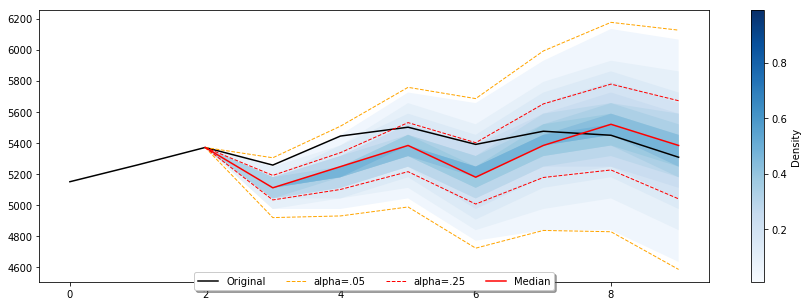
\includegraphics[width=6in,height=1.8in]{figures/arima.png}
\label{fig:arima}}
\end{subfloat}

\begin{subfloat}[Quantile Auto Regression - QAR]{
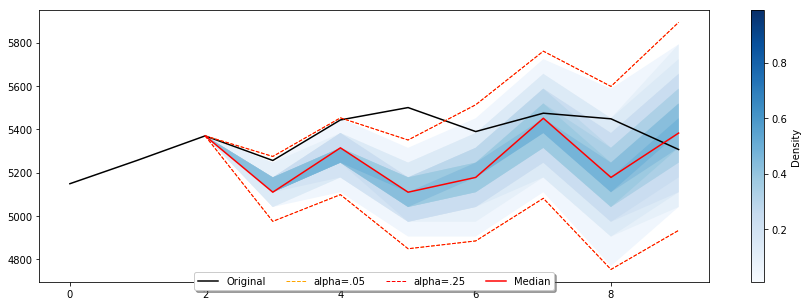
\includegraphics[width=6in,height=1.8in]{figures/qar.png}
\label{fig:qar}}
\end{subfloat}

\begin{subfloat}[Bayesian Structural Time Series - BSTS]{
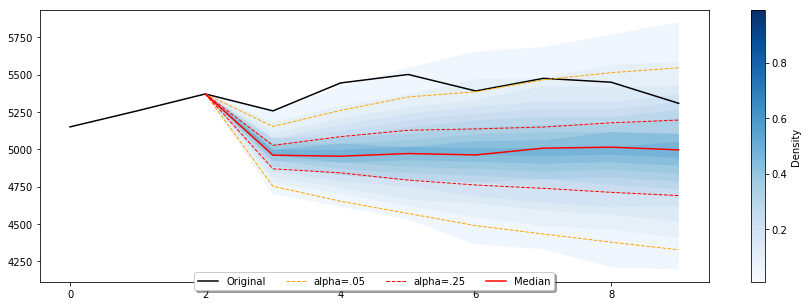
\includegraphics[width=6in,height=1.8in]{figures/bsts.png}
\label{fig:bsts}}
\end{subfloat}

\begin{subfloat}[k-Nearest Neighbors with Kernel Density Estimation - kNN/KDE]{
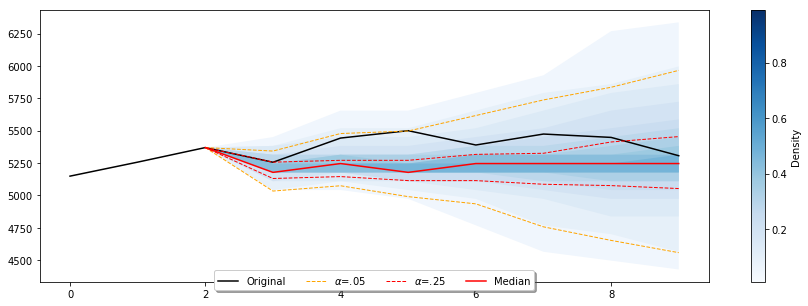
\includegraphics[width=6in,height=1.8in]{figures/knn.png}
\label{fig:knn}}
\end{subfloat}

\caption{Prediction Intervals}
\label{fig:prediction_intervals}
\end{center}
\end{figure*}

The Pinball Loss Function $\rho_\tau(u)$ is a general measurement to quantile approximation and \cite{Steinwart2011} also use it with Support Vector Machines to perform quantile regressions. \cite{Wan2014} use it with Extreme Learning Machines to fit quantile regression models. Other approaches are available in \cite{Takeuchi2006} for non parametric quantile estimation,  \cite{Taylor2007} proposes a Exponentially Weighted Quantile Regression and \cite{Hansen2006}, which proposes a semi-parametric k-step ahead approach for quantile estimation. \cite{Gardner1998} proposed a simple non parametric method for computing intervals based on the Chebyshev Inequality $P(|(Y-\mu)/\sigma|\geq \epsilon) \leq 1/\epsilon$ where $\mu$ is the mean, $\sigma$ the standard deviation and $\epsilon$ will be estimated value, such as the forecasted interval is $[y(t+1) - \epsilon, y(t+1) + \epsilon]$.

%%%%%%%%%%%%%%%%%%%%%%%%%%%%%%%%%%%%%%%%%%%%%%%%%%%%
%
%%%%%%%%%%%%%%%%%%%%%%%%%%%%%%%%%%%%%%%%%%%%%%%%%%%%
\subsection{Accuracy Measures for Interval Forecasts}
\label{sec:prob_interval_measures}
\index{Accuracy Measures}

In a wide sense the point forecasting accuracy measures can be used to assess the interval forecasts. This is possible by using the midpoint of the prediction interval, if the interval is based on $\alpha$-levels or symmetric quantiles. But, by far, this is not the ideal way to measure the interval accuracy, once several aspects of prediction intervals are neglected by single point measures.

Some of the main aspects to be considered when evaluating prediction intervals are the \textit{coverage rate}, \textit{calibration} and \textit{sharpness}, as proposed in \cite{Gneiting2007} and \cite{Pinson2006}. The \textit{coverage} refers to the statistical consistency between the forecasts and the observations, and measures which proportion of the observations are inside the interval. This can be done by an Indicator Function, developed by \cite{Christoffersen1998}, as shown in Equation \eqref{eqn:indicator}. Given a forecasting interval $\interval, u,l \in U$ and the real value $y\in Y$, the value of an indicator function $\mathbf{1}(\intvl(t),y(t))$ verifies if $y(t)$ is covered by $\intvl(t)$ or not.

\begin{equation}
\mathbf{1}(\intvl(t),y(t)) = \left\{ \begin{array}{cl}
1 & \text{if }y(t) \in \intvl(t) \\
0 & \text{if }y(t) \ni \intvl(t) 
\end{array} \right.
\label{eqn:indicator}
\end{equation}

\index{Coverage Rate}\index{Interval metrics}

The \textit{coverage rate} is the average value of indicator function between forecasted intervals and the real values, in which the ideal value is 1. The coverage rate is shown at Equation \eqref{eqn:coverage} where $y(t) \in Y$ are the real values and $\intvl(t) \in \intvl$ are the predicted intervals for these values.

\begin{equation}
C(Y,\intvl) = T^{-1}\sum_{t = 1 }^T \mathbf{1}(\intvl(t),y(t))
\label{eqn:coverage}
\end{equation}

\index{Sharpness}\index{Resolution}\index{Interval metrics}

The property of \textit{sharpness} and \textit{resolution} refers to the concentration of the predictive distribution, or how wide and variable are the intervals and refers uniquely to the forecasts. \textit{Sharpness}, presented in Equation \eqref{eqn:sharpnes}, is the average size of the intervals and \textit{resolution}, presented in the equation \eqref{eqn:resolution}, is the variability of the intervals.   

\begin{equation}
\overline{\delta(\intvl)} = T^{-1}\sum_{t=1}^{T} \delta(\intvl(t)) =  T^{-1}\sum_{t=1}^T \overline{u_t} - \underline{l_t}
\label{eqn:sharpnes}
\end{equation}
\begin{equation}
\sigma(\intvl) = T^{-1}\sum_{t=1}^T | \delta(\intvl(t)) - \overline{\delta(\intvl)}|
\label{eqn:resolution}
\end{equation}

While small values of $\overline{\delta(\intvl)}$ are desirable, meaning a compact interval, wide values of $\sigma(\intvl)$ are best, meaning the capability of the model to adapt the length of interval with the increase of uncertainty. There are no absolute reference values for sharpness and resolution, which depend on the statistical properties of the data. Empirically, when the sharpness is reduced to make the intervals thinner and more precise, the risk of reducing the coverage increases, and that's why the resolution is important. 

\index{Pinball Loss Function}\index{Pinball Score}\index{Interval metrics}

\cite{Steinwart2011} proposed the use of Pinball Loss Function - $\rho_\tau(u)$, defined in Equation \eqref{eqn:pinball} where $u = y(t) - \hat{y}(t)$, to indicate the proximity of a forecast $\hat{Y}$ with a certain $\tau$ quantile of the true value $Y$. As a loss function, the minor value of $\rho_\tau$ indicates the closest forecast to quantile $\tau$. The Pinball Score $\rho_\tau^S$ is defined as the mean $\rho_\tau$ for a set true values $y(t)$ and forecasts $\hat{y}(t)$, listed in Equation \eqref{eqn:pinball_score}. At this research the quantiles $\tau = \{0.05, 0.25, 0.75, 0.95\}$ were chosen for testing the intervals, where the lower quantiles were compared with the interval lower bound and the upper quantiles with the interval upper bounds.

\begin{equation}
\rho_\tau^S(Y,\hat{Y}) = \frac{1}{T}\sum_{t=1}^T \rho_\tau(y(t) - \hat{y}(t))
\label{eqn:pinball_score}
\end{equation}

However, using three separate metrics make the analysis of interval forecasters more complex. The most common option in these cases is the Winkler score \cite{winklerscore}, which encompasses the three characteristics in only one measure. Given a target value $y$ and a prediction interval $\interval$ with nominal probability $(1 - \alpha)$, the Winkler Score (WS) is defined by  \eqref{eqn:winkler}, where $\delta = \overline{u} - \underline{l}$. The score value is the interval width, but it increases when the target value is not covered by the interval and the penalty is proportional to the error given the nominal probability. Lower values therefore represent better prediction intervals. The mean score is defined by Equation \eqref{eqn:mean_winkler}, where $T$ is the sample size.

\begin{equation}
WS(\alpha, y(t), \intvl(t)) = \left\{ \begin{array}{ccl}
\delta & if & \underline{l} \leq y \leq \overline{u} \\
\delta + 2(\underline{l} - y)/\alpha & if & y < \underline{l}  \\
\delta + 2(y - \overline{u})/\alpha & if & \overline{u} < y   
\end{array} \right.
\label{eqn:winkler}
\end{equation}

\begin{equation}
\overline{WS(\alpha, Y, \intvl)} = T^{-1} \sum_{t=1}^T S(\alpha, y(t),\intvl(t))
\label{eqn:mean_winkler}
\end{equation}

All revised interval forecasting methods are based on non-FTS methods and this is a gap in the FTS literature. In the next section a method for quantifying the bounds of fuzzy uncertainty is proposed.

%%%%%%%%%%%%%%%%%%%%%%%%%%%%%%%%%%%%%%%%%%%%%%%%%%%%
%
%%%%%%%%%%%%%%%%%%%%%%%%%%%%%%%%%%%%%%%%%%%%%%%%%%%%
\section{The Interval Fuzzy Time Series  - $\ifts$}\index{Interval Fuzzy Time Series}\index{$\ifts$}
\label{sec:ifts}

This section proposes the Interval Fuzzy Time Series ($\ifts$), a simple, fast and effective method to deal with fuzzy empirical uncertainty, combining the flexibility of the FTS models with the properties of Interval Forecasts without the need to resort to parametric methods or optimization techniques as in quantile estimation methods.

It was already discussed in Section \ref{sec:fts_partitions} the impact of the number of partitions $k$ on the accuracy of a FTS model. Also, in Section \ref{sec:fts_defuzzyfication} it can be seen that in the deffuzification process only the midpoint of each fuzzy set is taken into account. This leads to the following question: what is the impact of the fuzzy set uncertainty (due to the overlapped bounds of the fuzzy set) on the final forecasting uncertainty? Since  the fuzzy sets represent the empirical uncertainty of $Y$, how this uncertainty is propagated to the point forecasts?

 The main advantage of the proposed method is to keep the model fast and scalable, for instance when the method is used in a high volume data or on a fast stream with concept drifts, which demands the model to be frequently updated. The scalability of FTS models will be discussed with more details in Chapter \ref{chap:scalability}.

The Interval Fuzzy Time Series Model ($\ifts$) aims to produce a prediction interval that represents the empirical uncertainty caused by the number of partitions $k$ and the fuzzy sets bounds, but without any probabilistic meaning. The method $\ifts$ is a time invariant, rule based and high-order method that just  introduces a new deffuzyfication type on forecasting procedure, without modifying the training method and, because of this, it can be applied to every conventional FTS method.  

The model training procedure is the same of HOFTS presented in Section \ref{sec:fts_training_procedure} and aims to construct the FLRG rule base $\model$. The prediction intervals are based on the mean interval of the $RHS$ fuzzy sets on each FLRG weighted by their fuzzy membership in relation to input value.

In the following section the forecasting method of $\ifts$ will be presented, it extends the HOFTS forecasting method, presented in Section \ref{sec:fts_forecasting_procedure}, changing its output from the crisp value $\estimate$ to the prediction interval $\intvl(t+1)$.

%%%%%%%%%%%%%%%%%%%%%%%%%%%%%%%%%%%%%%%%%%%%%%%%%%%%
%
%%%%%%%%%%%%%%%%%%%%%%%%%%%%%%%%%%%%%%%%%%%%%%%%%%%%
\subsection{Forecasting Procedure} \index{Forecasting Procedure} 
\label{sec:ifts_forecasting_procedure}

\begin{enumerate}
\item [Step 1] \textit{Fuzzyfication}: Compute the membership grade $\mu_{ti}$ for each $y(t) \in Y$ where $t \in L$ and each fuzzy set $A_i \in \Tilde{A}$, such that $\mu_{ti} = \mu_{A_i}(y(t))$. 
\item [Step 2] \textit{Rule matching}: Select the $K$ rules where all fuzzy sets $A_i$ on the LHS have $\mu_{ti} > \alpha$; The rule fuzzy membership grade is shown below, using the minimum function as T-norm.
\begin{equation}
    \mu_j = \min_{t\in L\; i \in \Tilde{A}} \mu_{ti}
\end{equation}
\index{T-norm}\index{Triangular norm}
\item [Step 3] \textit{Interval Defuzzyfication}:
\begin{enumerate}
\item \textit{Rule intervals}: Each chosen rule $j$ will generate an interval $\mathbb{I}^j = [\underline{\mathbb{I}^j_{min}}, \overline{\mathbb{I}^j_{max}}]$ where $\mathbb{I}^j_{min}$ is the minimum lower bound of all RHS fuzzy sets of the rule $j$ and $\mathbb{I}^j_{max}$ is the maximum upper bound of RHS fuzzy sets of rule $j$;
\begin{equation}
\begin{array}{lcr}
\mathbb{I}^i_{min} & = & \min( A_1, ..., A_k ) \\
\mathbb{I}^i_{max} & = & \max( A_1, ..., A_k ) \\ 
& & A_1, ..., A_k \in RHS 
\end{array}
\label{eqn:iminimax}
\end{equation}

\item \textit{Final Prediction Interval}: The final forecast interval $\mathbb{I}(t+1)$ is calculated as the sum of the rules intervals weighted by the membership value of each rule, as shown in Equation \eqref{eqn:ifts}
\begin{equation}
\mathbb{I}(t+1) = \frac{\sum_{j \in A} \mu_i \mathbb{I}^j}{\sum_{j \in A} \mu_j} = \frac{\sum_{j \in A} [\mu_j\underline{\mathbb{I}^j_{min}} , \mu_j\overline{\mathbb{I}^j_{max}}] }{\sum_{j \in A} \mu_j}
\label{eqn:ifts}
\end{equation}
\end{enumerate}
\index{Many steps ahead forecast}
\item[Step 5] \textit{Many steps ahead forecast}:If the forecasting horizon is $H > 1$, define $\intvl_H = \{\intvl(t+1)\}$ as the set of intervals and repeat the steps below for each $h=2..H$, otherwise return  $\intvl(t+1)$.
\begin{enumerate}
    \item[a)]  Given $\intvl(t+h-1)= [\underline{l},\overline{u}]$, call recursively the forecasting method, such that $\intvl_l = forecast(\underline{l})$ and $\intvl_u = forecast(\overline{u})$. The interval $\intvl(t+h)$ is given by:
    \begin{equation}
        \intvl(t+h)= [\underline{min(\intvl_l)},\overline{max(\intvl_u)}]
    \end{equation}
    \item[b)] Append $\intvl(t+h)$ to $\intvl_H$ and if $h = H$ then return $\intvl_H$.
\end{enumerate}
\end{enumerate}

The generated interval $\intvl(t+1)$ is bounded by a composition of the fuzzy sets bounds on the FLRG's which have some membership with the input value $y(t)$ and is expected to contain the true value $\estimate$. A sample of the method performance, for one and many steps ahead, can be seen in Figures \ref{fig:ifts_sample_onestep} and \ref{fig:ifts_sample_manystep}. In the next section a weighted version of $\ifts$ is presented. 

\begin{figure}[htb]
    \centering
    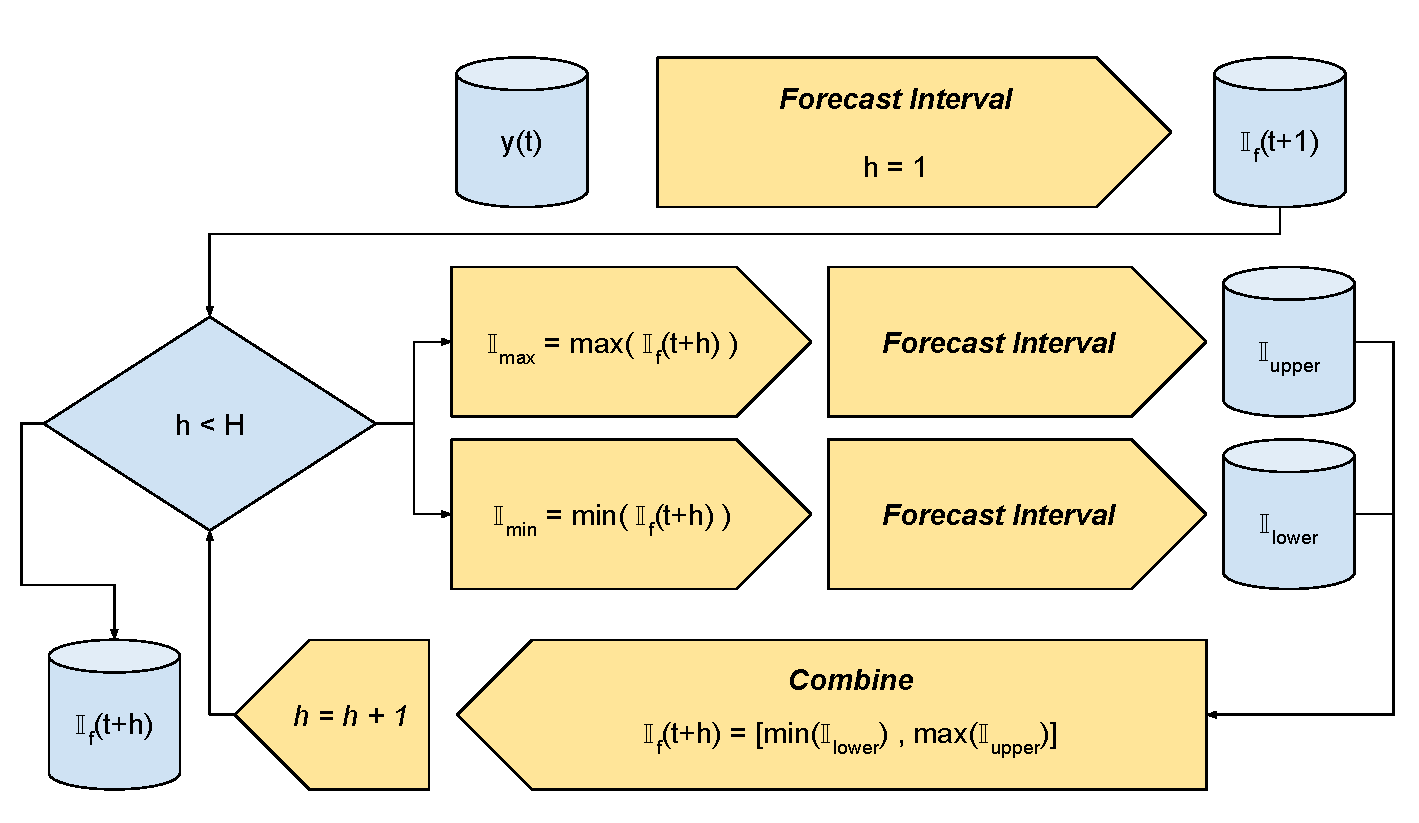
\includegraphics[width=\textwidth]{figures/ifts_many_steps.pdf}
    \caption{$\ifts$ many steps ahead interval forecasting procedure}
    \label{fig:ifts_many_steps}
\end{figure}

%%%%%%%%%%%%%%%%%%%%%%%%%%%%%%%%%%%%%%%%%%%%%%%%%%%%
%
%%%%%%%%%%%%%%%%%%%%%%%%%%%%%%%%%%%%%%%%%%%%%%%%%%%%
\subsection{Weighted $\ifts$}\index{$W\ifts$}\index{Weighted $\ifts$}
\label{sec:wifts}

A weighted $\ifts$ extension uses the same model building procedure  of WHOFTS method, presented in Section \ref{sec:fts_whofts} and aims to construct the weighted FLRG rule base $\model$. The prediction intervals are based on the weighted interval of the $RHS$ fuzzy sets on each FLRG weighted by their fuzzy membership in relation to input value.

$W\ifts$ extension also changes the Steps 3.a of the Forecasting Procedure, replacing the Equation \eqref{eqn:iminimax} by the Equation \eqref{eqn:weighted_iminimax}, where $\underline{\ufset}$ and $\overline{\ufset}$ represents respectively the lower and upper bounds of each fuzzy set $\ufset \in RHS$:

\begin{equation}
\begin{array}{ccc}
\intvl_{min} & = & \sum_{j \in RHS} w_j \cdot \underline{\ufset} \\
& & \\
\intvl_{max} & = & \sum_{j \in RHS} w_j \cdot \overline{\ufset}
\end{array}
\label{eqn:weighted_iminimax}
\end{equation}

\begin{figure}[htb]
    \centering
    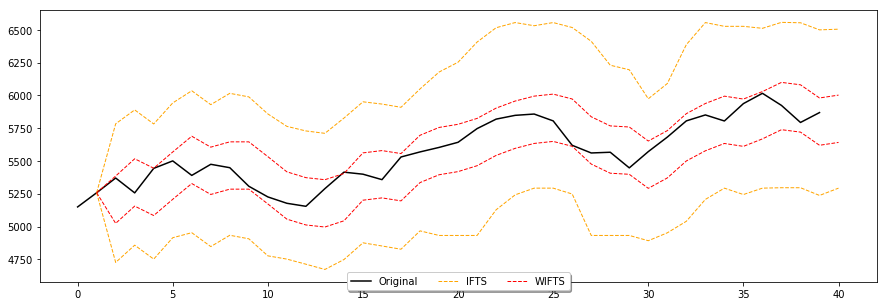
\includegraphics[width=\textwidth]{figures/ifts_sample_onestep.png}
    \caption{Sample of $\ifts$ and $W\ifts$ methods for one step ahead}
    \label{fig:ifts_sample_onestep}
\end{figure}

\begin{figure}[htb]
    \centering
    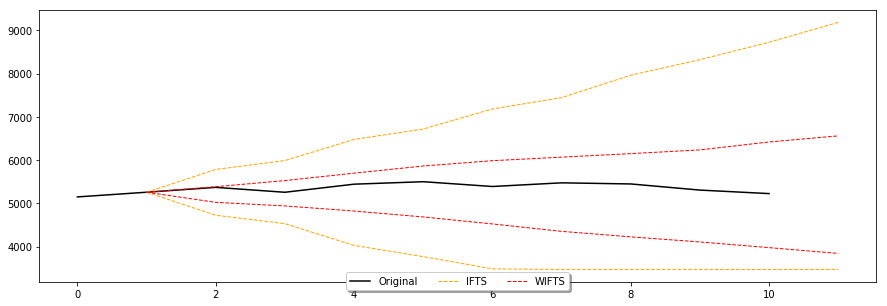
\includegraphics[width=\textwidth]{figures/ifts_sample_manystep.png}
    \caption{Sample of $\ifts$ and $W\ifts$ methods for many steps ahead}
    \label{fig:ifts_sample_manystep}
\end{figure}

Different from $\ifts$, which considers the extremum of the fuzzy sets, the generated interval $\intvl(t+1)$ of $W\ifts$ is bounded by a weighted composition of the fuzzy sets bounds, making it more sharper. A sample of the method performance, for one and many steps ahead, can be seen in Figures \ref{fig:ifts_sample_onestep} and \ref{fig:ifts_sample_manystep}. 

Interval forecasts help to embrace the notion of forecast uncertainty, but did not offer a complete landscape of the uncertainty. In the next sections, the probabilistic forecasting is presented as a more embracing way to represent the uncertainty.

%%%%%%%%%%%%%%%%%%%%%%%%%%%%%%%%%%%%%%%%%%%%%%%%%%%%
%
%%%%%%%%%%%%%%%%%%%%%%%%%%%%%%%%%%%%%%%%%%%%%%%%%%%%
\section{Probability Distribution Forecasts}\index{Probability Distribution Forecasts}
\label{sec:prob_distribution}

If the interval forecast represents a range of uncertainty, according to \cite{Krzysztofowicz2001} the probabilistic distribution forecast ``should quantify the total uncertainty that remains about the predictand, conditional on all information utilized on the forecasting process''. 

The probability distribution forecasts cover the complete range of the $U$ and can be continuous, using a probability density function, or discrete using both a discrete probability mass function or an empirical probability distribution, as histograms. In this last case, $U$ is split in $n$ equal length sub-intervals $b_i$ - called bins -, which are associated to a probability $p_i$ of occurrence, such as $\sum_{i=1}^n p_i = 1$. The length of each bin is the unit of discretization also referenced as the resolution of the distribution. 

Probability distribution forecasts can be represented also as the empirical cumulative probability distribution function $F(x) = n^{-1}\sum_{i\in Y(t)} \mathbf{1}(i < x)$ where $\mathbf{1}(c) = \{1$ if $c = True;\ 0,$ otherwise $\}$. Using $\alpha$-level prediction intervals, described in Section \ref{sec:prob_interval}, for $\alpha \in [0.05, ..., 0.5]$, it is easy to construct the empirical distribution $F$ by iteration over the bounds of intervals. This approach was used to produce the distributions in Figure \ref{fig:arima}, from 7-steps ahead mean-variance prediction intervals over an ARIMA(2,0,0) model. The same approach can be used to construct probabilistic forecastings using QAR method, as shown in Figure \ref{fig:qar}.

\index{Gaussian Process Regression}\index{GPR}

The Gaussian Process Regression (GPR), as discussed in \cite{Rasmussen2006} and \cite{Roberts2013}, is an instance based parametric approach which interpolates the instances $y(t) \in Y$ and also produces an extrapolation for $y(t+1)$ in the form of a Gaussian Distribution. A Gaussian Process $\mathcal{GP}(m,\kappa)$ is defined by a mean function $m(Y)$ and covariance kernel $\kappa(y(i),y(j))$ which produce the covariance matrix $\Sigma$, such that $y(t+1) \sim \mathcal{N}(m(Y),\Sigma)$. The mean function $m(Y)$ is defined as the unconditional expectation of $Y$, such that $m(Y) = \mathbb{E}[Y]$. The covariance matrix $\Sigma$ assigns the similarity $\sigma_{ij} \in \Sigma$ between all pairs of instances of the time series, and it is defined by the covariance function $\sigma_{ij} = \kappa(y(i),y(j))$ for all $i,j = 1..T$. The covariance function is defined as $\kappa: U,U \rightarrow \mathbb{R}^+$ and measures the similarity between the two instances. 

The covariance function $\kappa$ is the most important parameter of $\mathcal{GP}$ model, and it is responsible to measure how the instances relate with themselves and with time. $\kappa$ is usually defined by a set of parameters or hyperparameters $\theta$, and because this $\kappa$ is also often written as $\kappa(y(i),y(j)|\theta)$ to make the dependence on $\theta$ explicit. 

The most notable drawbacks of the GPR approach are the parametric assumption, the non-sparsity, i.e., it uses the whole set of samples to perform one prediction which is undesirable for Big Data scenarios. Even with the fast and direct aproaches developed by \cite{Ambikasaran2014}, that method still loses efficiency as the number of variables grows.

\index{Bayesian Methods}\index{Bayesian Structural Time Series}\index{Space-State Models}

The Bayesian Structural Time Series (BSTS), discussed in \cite{Scott2014} and \cite{Barber2011a}, mix the well known State-Space models with the Bayesian Statistics approach for parameter estimation. A structural time series is a state-space model which associates the observed value $y(t)$ with an unobserved latent state  $s_t$. The structure is defined by a system of equations where the observation equation (also known as measurement equation) is defined in Equation \eqref{eqn:observation} and the transition equation is defined in Equation \eqref{eqn:transition}, and this system of equations can also be referred as a Linear Gaussian Model. 
\begin{align}
    y(t)  = & Z_ts_t + \epsilon_t & \epsilon_t \sim \mathcal{N}(0, H_t) \label{eqn:observation} \\
    s_t  = & T_t s_{t-1} + R_t\eta_t & \eta_t \sim \mathcal{N}(0, Q_t)  \label{eqn:transition}
\end{align}

An observed value $y(t)$ is understood as a signal with noise, where the signal is the product of the unobserved state $s_t$ by the regressor parameter $Z_t$, and the noise (the extrinsic uncertainty) represented by the Gaussian error term $\epsilon_t$ whose variance is controlled by the parameter $H_t$. The unobserved latent state $s_t$ is represented by a vector with the several components of the time series, as trend, seasonality, level, etc, and is recursively defined by the transition matrix $T_t$ and the Gaussian error term $\eta_t$ (the intrinsic uncertainty), which in turn is controlled by the vector $R_t$ and the covariance matrix $Q_t$. The error terms $\epsilon_t$ and $\eta_t$ are mutually independent. This state-space representation can unify several approaches of time series forecasting and the parameters $Z_t,T_t,H_t,R_t$ and $Q_t$ define the structure of the model, hereafter called as the $\Theta$ or the parameter space. For instance, for an ARMA approach the regressors are represented by $Z_t$ and the coefficients by $T_t$. 

Once the state space model is defined, it is necessary to infer the values of $\Theta$ parameters from the training data $Y$, keeping in mind that $Y$ is a sample and it is composed with several sources of uncertainty, so it will be also $\Theta$. The Bayesian framework is employed in this task, which represents all uncertainties as probability distributions, from the learning process, passing through the parameter space $\Theta$, to the prediction space $U$. In such approach, the model parameters are probability distributions $P(\Theta|Y)$, reflecting the uncertainty around the real (but unknown) values of each parameter in $\theta \in \Theta$ given the learning sample $Y$. The forecast of $\estimate$ is a probability distribution $P(y(t+1)|\Theta,Y)$ that reflects the intrinsic uncertainty inherent of the time series $Y$, and the extrinsic uncertainty of the unknown real parameter values $P(\Theta|Y)$. 

The learning of the parameter space $\Theta$ is guided by the Bayes Rule. It states that, given a set of known evidences $d \in \mathcal{D}$ and a set of possible hypothesis $h \in \mathcal{H}$, the posterior distribution $P(h|\mathcal{D})$ is given by the Equation \eqref{eqn:bayes}, where $P(\mathcal{H})$ is the prior distribution, the $P(\mathcal{D}|h)$ is the likelihood, and $P(\mathcal{D})$ is the normalizing term, such that $P(\mathcal{D}) = \sum_{h \in \mathcal{H}}P(\mathcal{D}|h)P(h)$ according to the Law of Total Probability. 

\begin{equation}
    P(h|\mathcal{D}) = \frac{P(\mathcal{D}|h) P(h)}{P(\mathcal{D})} = \frac{P(\mathcal{D}|h) P(h)}{\sum_{h \in \mathcal{H}}P(\mathcal{D}|h)P(h)}
    \label{eqn:bayes}
\end{equation}

The prior distribution $P(\mathcal{H})$ assigns the knowledge about the chances of each $h \in \mathcal{H}$ be the real value. The likelihood function $\mathcal{L}(h|\mathcal{D})$ assembles the plausibility of the evidences $d \in \mathcal{D}$ to have been generated by the parameter $h$, and it is equals to $P(\mathcal{D}|h)$.

Some methods are available to estimate the best hypothesis $h$ in the search space $\mathcal{H}$. The Maximum A Posteriori (MAP) principle poses the best hypothesis $h \in \mathcal{H}$ is that one for which $h_{MAP} = \arg\max_\mathcal{H} P(h|\mathcal{D})$. Given that $P(\mathcal{D})$ is a constant and it is hard to compute, it is eliminated from the calculation, considering just $P(h|\mathcal{D}) \propto P(\mathcal{D}|h) P(h)$. The $h_{MAP}$ is used to update $P(\mathcal{H})$ and improve the aproximation of $P(\mathcal{H}|\mathcal{D})$ as new data is acquired. The Maximum Likelihood Estimation (MLE) method uses the average log-likelihood function $\hat{\mathcal{L}}(h|\mathcal{D}) =  |\mathcal{D}|^{-1}\sum_{i=0}^{|\mathcal{D}|} ln P(d_i|h)$ as a cost function, such that $h_{MLE} = \arg\max_\mathcal{H} \hat{\mathcal{L}}(h|\mathcal{D})$ is the best estimate parameter $h\in\mathcal{H}$. The drawback of these estimators is to estimate a unique point value without representing the uncertainty around the best hypothesis in $\mathcal{H}$.

However, the great strength of the Bayesian Methods is its ability to represent the uncertainties contained both on data and model parameters with probability distributions. This is also the great drawback of Bayesian Methods: their expensive computational cost. It is mainly because not all parts of its equation are always available -- like the likelihood function $P(\mathcal{D}|h)$ -- and those values needs to be simulated using Monte Carlo methods.

\index{Monte Carlo Methods}

The Monte Carlo (MC) methods, initially proposed in \cite{Metropolis1949}, are techniques to solve complex  integration problems using random sampling. They aim to generate a set of samples $x_1,\ldots,x_n$ from a target distribution $\pi(x)$ in order to estimate some hard-to-compute feature $\phi(x)$ using the expected value $\mathbb{E}[\phi(x)] = n^{-1}\sum_i^n \phi(x_i)$ which converges to the unobserved real value of $\phi$. Given the estimated value as $\overline{\phi} = \mathbb{E}[\phi(x)]$, and its variance as $\phi_\sigma = Var[\phi(x)]$, some statistical concepts support the convergence of the MC methods. The Law of Large Numbers (LLN) asserts that, for a large enough number of samples $n$, the difference between the estimated value $\overline{\phi}$ and the true value $\phi$ decays to zero, or $P(\lim_{n\to\infty} |\overline{\phi} - \phi| = 0) = 1$ . The Central Limit Theorem (CLT) states that, for a large enough number of samples $n$, the $\overline{\phi}$ is normally distributed as $\overline{\phi} \sim \mathcal{N}(\phi,\phi_\sigma/n)$.

\index{Markov Chain Monte Carlo}\index{MCMC}

Markov Chain Monte Carlo (MCMC) methods improve the basic MC approach aiming to, instead of sampling $\pi(x)$ directly, sample from a Markov Chain with a transition matrix $K$, where $K_{i,j} = P(x_t = i|x_{t-1} = j)$, such that the next sample $x_t$ be conditionally dependent on the previous $x_{t-1}$. The Markov Chain $K$ needs to approximate the real $\pi(x)$ distribution, but estimating $K$ is very often an intractable problem. An approximation is provided by the Metropolis-Hastings algorithm generalized in \cite{Hastings1970}, which provide a simple and efficient way to simulate $K$ and generate samples. 

Estimating $P(\Theta|Y)$ using Bayesian methods is an optimization task which employs MCMC in order to sample from $P(Y|\Theta)P(\Theta)$ distribution, while refining the parameters of $P(\Theta)$. The method demands the choice of an appropriate a priori distribution $P(\Theta)$ that will rule the search space of each parameter $\theta \in \Theta$. The likelihood $P(Y|\Theta)$ estimates the fit of each parameter $\theta \in \Theta$ when generating samples of $y(t)\in Y$. This likelihood is itself another challenge once the samples $y(t)\in Y$ may be identically distributed but are not independent, there is a temporal dependence between $y(t)$ and it's past lags $y(t-1),...$ that must be respected. This problem demands the use of advanced MCMC methods as Sequential Monte Carlo, Sequential Importance Sampling and Particle Filters, deeply discussed in \cite{Smith2013}.

Once $\Theta$ values were estimated and represented by probability distributions $P(\Theta|Y)$, the estimation of $\estimate$ will be represented by a probability distribution $P(y(t+1)|\Theta,Y)$, defined in Equation \eqref{eqn:posteriori}, which is also expensive to calculate and, again, needs to resort to MCMC methods. 

\begin{equation}
    P(y(t+1)|\Theta,Y) =  \int_U \int_\Theta P(y|\theta,Y)P(Y|\theta)P(\theta) dy d\theta
    \label{eqn:posteriori}
\end{equation}

A small sample of the BSTS method is shown in Figure \ref{fig:bsts}, for 7 steps ahead interval and probabilistic forecasting. If in one hand the Bayesian Structural Time Series are well succeeded in representing the intrinsic and extrinsic uncertainties, on the other hand it is complex to implement and computationally expensive to run, making it not applicable for a variety of scenarios where the time performance is mandatory.

\index{Forecast Combination}\index{Ensemble Forecasting}\index{Ensemble Learning}\index{Ensemble Models}

There are other approaches to embody the  uncertainties of model parameters. Monte Carlo methods itself evoke the idea of forecasting combination and Ensemble Methods, as posed in \cite{Smith2001}, ``In practice, ensemble forecasting is a Monte Carlo approach to estimating the probability density function (PDF) of future model states given uncertain initial conditions''. Forecast combination is not a new concept, see \citep{Clemen1989}, and start from the idea to mix different sources to improve forecasting. This is sightly close to the concept of Ensemble Methods defined by \cite{Gneiting2008} as ``an ensemble prediction system consists of multiple runs of numerical weather prediction models, which differ in the initial conditions''. Also \cite{Leutbecher2008} states that ``The ultimate goal of ensemble forecasting is to predict quantitatively the probability density of the state of the atmosphere at a future time''. 

Initially Ensemble Learning methods were developed to produce point forecasts as combination of the individual model's forecasts by a weighted average or more complex methods as Bayesian Model Averaging, for instance  \cite{Raftery2005}. Soon after, these methods were adapted for probabilistic forecasting as in \cite{Gneiting2005}, \cite{Leutbecher2008} and \cite{Fraley2013}. \cite{Xie2016} proposed a methodology for electric load probabilistic forecasting in three steps: \textit{pre-processing step} consisting of data cleaning;  \textit{forecasting step} using point-forecasting methods, forecast combination and scenario-based probabilistic forecasting; \textit{post-processing step} performing a simulation on the residuals of the selected point forecasting models in order to improve the probabilistic forecast.

These ensembles can be homogeneous (same method with different parameters) or hybrid (different methods with different parameters). This set of models $\mathcal{M}$ receive a set of parameters $\Theta$ to produce a set of forecasts $\estimate$, such as $\estimate^i = m_i(\theta_i)$, $\forall m_i \in \mathcal{M}$ and the $\theta_i\in \Theta$ values are drawn of a prior probability distribution $P(\Theta)$. The methods can be executed several times and the larger the sample is, the better approximations are made. After $n$ runs, the empirical distribution $P(y(t+1))$ of the outputs is available.

Ensemble Learning is a variation of the Ensemble Forecasting on Machine Learning field, defined by \cite{Brown2010} as ``the procedures employed to train multiple learning machines and combine their outputs with individual predictions combined appropriately, should have better overall accuracy, on average, than any individual committee member''. Ensemble Learning can be used in classification in regression tasks, also time series forecasting as in \cite{Chen2005}, \cite{Bai2010} and \cite{Koskova2015a}.

This concept is exploited in \cite{Mohammed2015} and \cite{Mohammed2016},  which proposed an ensemble learning approach for solar power probabilistic forecasting based on k-Nearest Neighbors, Regression Trees, Random Forests and regression methods. Given an ensemble with $k$ models and taken the ordered set of the $k$ individual forecasts, the probabilistic forecast is constructed as an empirical cumulative distribution $F$, calculated with the percentiles of the individual forecasted values. $F$ can be made with three approaches: \textit{quantile linear interpolation}, \textit{normal distribution} and \textit{normal distribution with initial different conditions}. The linear interpolation approach calculates the $\tau$ quantile position $r_\tau$ on the individual forecasts as $r_\tau = \frac{k\tau}{100}+0.5$. The normal distribution approach is similar to mean-variance model of section \ref{sec:prob_interval}. With the set of individual forecasts the mean $\mu$ and the variance $\sigma$ are calculated, and the $\tau$ quantile is given by $\tau = \mu + z_\tau\cdot\sigma$. The third approach is specific for the application domain of solar power.

The advantage of \cite{Mohammed2015} approach is the flexibility and ease of implementation, since the individual models can be replaced (or added) for any other point forecaster, for instance, any FTS method. As more models are added to the ensemble, better will be the probabilistic distributions but also become more computationally expensive. 

\index{Kernel Density Estimation}\index{KDE}

Other distributions generating techniques for ensemble forecasts exist as Kernel Density Estimation \citep{Hong2016a} and Kernel Dressing [ \citep{Pinson2009} and \citep{Brocker2008}] and can be easily combined with instance-based methods as k-nearest neighbors. Both approaches smooth the discrete values in a continuous function that approximates the empirical distribution of data, as exposed in Equation \eqref{eqn:kde}, where $Y$ is the set of individual forecasts, $K$ is the kernel function and $h$ is a smoothing parameter also known as bandwidth.:

\begin{equation}
P(x) = (nh)^{-1} \sum_{i \in Y} K\left(\frac{x - i}{h}\right)
\label{eqn:kde}
\end{equation}

A kernel function $K$ have to be a non-negative, real-valued, symmetric, integrable and normalized, such that $\int_{-\infty}^{+\infty}K(u) du = 1$. A review of density estimation methods can be found in \cite{Silverman1986} and a specific study on estimation of $h$ parameter can be found in \cite{Sheather1991}. A small sample of the kNN with KDE approach is shown in Figure \ref{fig:knn}, for 7 steps ahead interval and probabilistic forecasting. 

\begin{table}[]
    \centering
    \begin{tabular}{|c|c|} \hline
        \textbf{Kernel} & \textbf{Definition} \\ \hline
        Triangular & $K(u) = 1 - |u|$ \\ \hline
        Tophat & $K(u) = \frac{1}{2}\mathbb{I}(|u| < 1)$ \\ \hline
        Epanechnikov & $K(u) = 3/4(1-u^2)$ \\ \hline
        Gaussian & $K(u) = \frac{1}{\sqrt{2\pi}}e^{-1/2u^2}$ \\  \hline
    \end{tabular}
    \caption{KDE Kernels}
    \label{tab:kde_kernels}
\end{table}

The several methods discussed in this section are spread in the literature. In the next section accuracy measures for probabilistic forecasting are discussed.

%%%%%%%%%%%%%%%%%%%%%%%%%%%%%%%%%%%%%%%%%%%%%%%%%%%%
%
%%%%%%%%%%%%%%%%%%%%%%%%%%%%%%%%%%%%%%%%%%%%%%%%%%%%
\subsection{Accuracy Measures for Probabilistic Forecasts}
\label{sec:prob_probabilistic_measure}
\index{Accuracy Measures}

As the probabilistic forecast provides the landscape of uncertainty for the whole $U$, it is also possible to use the accuracy measures presented in Sections \ref{sec:point_measures} and \ref{sec:prob_interval_measures} to assess its accuracy. A probability distribution can be reduced to a point using its expected value $\mathbb{E}$ or it's median $m = F(.5)$. In both cases, the point forecasting accuracy values can be used to assess its accuracy.

A probability distribution $P$ can also be expressed in terms of intervals as well, by using $\alpha$-levels and their respective quantiles. In this case, the prediction interval accuracy measures can be used to evaluate $P$ accuracy in several different $\alpha$, in the many different aspects discussed in Section \ref{sec:prob_interval_measures}.

But pure probabilistic accuracy measures intend to assess how well the probabilities of $P$ are spread over $U$ when we know the true value $y(t)$, and how close $P$ were able to predict the uncertainty around $y(t)$. The most simple probabilistic forecasting measure is the Logarithm Score (LS), proposed in \cite{Good1952} and defined in Equation \eqref{eqn:log_score}, which indicates how strong was the probability distribution $P$ to predict the real value $y(t)$. The Logarithm Score presents some limitations as, for instance, when $P(y(t)) = 0$ then $LS(P,y(t)) = \infty$.

\begin{equation}
    LS(P,Y) = T^{-1} \sum_{t=1}^T -log(P(y(t)))
    \label{eqn:log_score}
\end{equation}

\index{Brier Score}

The Brier Score (BS), proposed in \cite{Brier1950} and defined in Equation \eqref{eqn:brier_score}, was originally defined for $R$ categorical events but it is possible to extend it for numeric values by splitting the Universe of Discourse in $R$ bins, or to consider the quantiles. This score can be interpreted as the Mean Squared Error (MSE) from the predicted probabilities for each bin $r$, represented by $P(r)$, to the real observed events represented by $\mathbf{1}\{ y(t) \in r\}$.

\begin{equation}
    BS(P,Y) = T^{-1} \sum_{t=1}^T \sum_{r=1}^R ( P(r) - \mathbf{1}\{ y(t) \in r\})^2
    \label{eqn:brier_score}
\end{equation}

\index{Continuous Ranked Probability Score}\index{CRPS}\index{Probabilistic forecast metrics}

The metric chosen to assess the distributions is the Continuous Ranked Probability Score (CRPS). CRPS is a proper measure for probabilistic forecasts, defined by  \cite{Gneiting2007b} as Equation \eqref{eqn:crps1} for one forecast and by \cite{Gneiting2007b} as Equation \eqref{eqn:crps2} for more than one forecasts. CRPS provides a direct way to benchmark probabilistic forecast since it is expressed in the same unit as the observed variable and is a generalization of the Mean Absolute Error (MAE). Therefore, the perfect score for CRPS, as in MAE, is 0.

\begin{equation}
CRPS(F,x) = \int_{-\infty}^{+\infty} (F(y) - \mathbf{1}\{y \geq x\})^2  dy
\label{eqn:crps1}
\end{equation}

\begin{equation}
CRPS(F,x) = \frac{1}{N} \sum_{t=1}^{N} \int_{-\infty}^{+\infty} (F_t(y) - \mathbf{1}\{y \geq x_t\})^2  dy
\label{eqn:crps2}
\end{equation}
where $F$ is the cumulative distribution function (CDF) of the forecasted distribution, $x$ is the true value and $\mathbf{1}\{y \geq x\}$ is the Heavyside function representing the CDF of this punctual value.

%%%%%%%%%%%%%%%%%%%%%%%%%%%%%%%%%%%%%%%%%%%%%%%%%%%%
%
%%%%%%%%%%%%%%%%%%%%%%%%%%%%%%%%%%%%%%%%%%%%%%%%%%%%
\subsection{Fuzzy Time Series Methods With Probabilistic Background}
\index{Fuzzy Probabilistic Models}

The first studies to make the relationship of probabilities with fuzzy sets came from Prof. Zadeh, \cite{Zadeh1968}, \cite{Zadeh1984}, which defines the fuzzy set probability as the expectation of the membership function. Also, Klement, Schwyhla and Lowen \cite{ErichPeterKLEMENT1981} and \cite{Dubois1989} explore the relationships between the fuzzy membership functions and the probability measures based on Measure Theory. 

These theoretical works form the basis of the Fuzzy Stochastic Fuzzy Time Series (FSFTS) of Song, Leland and Chissom \cite{Song1997}, where three models were presented but there is no empirical analysis of their results. In their work the probability space $[0,1]$ is also described by a linguistic variable $\tilde{P}$ with few fuzzy sets that describe the probability in linguistic terms like ``low'',``medium'',``high''. The rules of the model are composed by tuples $(p_j,\ufset)$ where $p_j \in \tilde{P}$ and $\ufset \in \ulvar$ and the deffuzyfication weights the fuzzy sets by their fuzzy probability.

 \cite{Gangwar2014} proposed the \textit{Probabilistic and Intuitionistic Fuzzy Time Series} - PIFTS method, strongly based on data normality and explicit Gaussian Process assumption. \cite{Cheng2012} and \cite{Chuang2014} use the Song and Chissom relation matrix and a Hidden Markov Chains for generating simulations for forecasting step, the \textit{Probabilistic Smoothing Hidden Markov Model FTS} - psHMM-FTS, which has high computational cost.

%%%%%%%%%%%%%%%%%%%%%%%%%%%%%%%%%%%%%%%%%%%%%%%%%%%%
%
%%%%%%%%%%%%%%%%%%%%%%%%%%%%%%%%%%%%%%%%%%%%%%%%%%%%
\section{The Ensemble FTS Method}
\label{sec:ensemblefts}\index{EnsembleFTS}

This section proposes the EnsembleFTS, a method able to perform probabilistic forecasts based on ensemble forecasts with Kernel Density Estimation.

The $\ifts$ method, presented in Section \ref{sec:ifts}, represent the forecasting uncertainty using the mean of the bounds of the fuzzy sets, or the empirical uncertainty, without any probabilistic sense. However, the FTS methods use of several ways to represent the time series uncertainties, as the number of partitions $k$, order $\Omega$, lag indexes $L$, rule weights. There are uncertainties surrounding these values due to the ontological uncertainty of the data, uncertainties that will be reduced -- but not removed -- after the hyperparameter optimization  proposed in Chapter \ref{chap:scalability}.

\index{$\model$}\index{Hyperparameter}
A way to encompass these uncertainties is to generate a meta model $\model$, composed with several FTS models $m \in \model$, such that each one of these individual models is trained with different values of FTS hyperparameters, which aim to represent the hyperparameter uncertainty and its effects. The aggregation of the individual forecasts $\estimate_m$ produced by each $m \in \model$ can represent the overall probabilistic uncertainty $P$ over the possible values of $y(t+1) \in U$ using kernel density estimation seen in Section \ref{sec:prob_distribution}.

Several approaches can be adopted to represent the uncertainty of the hyperparameter, from varying the number of partitions and order, passing through varying the partitioning methods, until varying the FTS method itself. However, the present approach adopts a conventional rule-based high order FTS method with a Grid partitioning method, varying only the number of partitions $k$ and order $\Omega$.\index{Hyperparameter}

On EnsembleFTS the hyperparameters $k$ and $\Omega$ are intervals and not scalar values. During the training procedure, explained in Section \ref{sec:ensemblefts_training} an FTS model will be trained for each combination of individual values in the Cartesian Product of $k$ and $\Omega$. In the forecasting procedure detailed in Section \ref{sec:ensemblefts_forecasting}, the input sample is presented for all internal models and their outputs are aggregated using a KDE, producing a probability distribution $P:U \rightarrow [0,1]$. Besides $k$ and $\Omega$ ranges, the kernel function $K$ and its bandwidth parameter $h$ are also parameters of the model.

%%%%%%%%%%%%%%%%%%%%%%%%%%%%%%%%%%%%%%%%%%%%%%%%%%%%
%
%%%%%%%%%%%%%%%%%%%%%%%%%%%%%%%%%%%%%%%%%%%%%%%%%%%%
\subsection{Training Procedure}
\label{sec:ensemblefts_training}\index{Training Procedure}

The aim of the training procedure is to build an ensemble $\model$ with $k\times\Omega$ individual models $m_i$, given a crisp training set $Y$. The overall training procedure is shown in Figure \ref{fig:ensemblefts_training} and it is composed of the following steps:

\begin{figure}[htb]
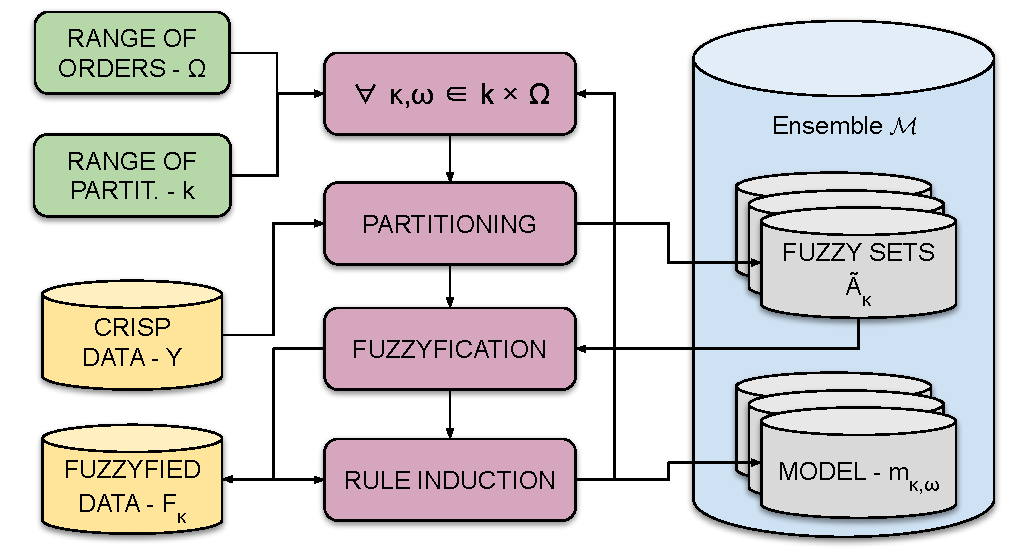
\includegraphics[width=\textwidth]{figures/ensemblefts_training.pdf}
\caption{Ensemble FTS training procedure}
\label{fig:ensemblefts_training}
\end{figure}

\begin{enumerate}
\item[Step 1] \textit{Main Loop}: For each pair $(\kappa,\omega)$ created by the cartesian product of each $\kappa \in k$ with each $\omega \in \Omega$, repeat Steps 2 to 5;
\item[Step 2] \textit{Partitioning}: Create a linguistic variable $\ulvar_\kappa$ over $U$ with $\kappa$ fuzzy sets using the Grid partitioning method and triangular $\mu$;
\item[Step 3] \textit{Fuzzyfication}: Fuzzyfy the crisp time series $Y$ using the linguistic variable $\ulvar_\kappa$, creating the fuzzyfied time series data $F_\kappa$;
\item[Step 4] \textit{$\omega$-order model}: With $F_\kappa$, use the high order weighted rule knowledge model to infer  $\omega$-order fuzzy rules and compose the model $m_{\kappa,\omega}$;
\item[Step 5)] \textit{Ensemble}: Append the model $m_{\kappa,\omega}$ on $\model$;
\end{enumerate}
\index{Ensemble Models}

%%%%%%%%%%%%%%%%%%%%%%%%%%%%%%%%%%%%%%%%%%%%%%%%%%%%
%
%%%%%%%%%%%%%%%%%%%%%%%%%%%%%%%%%%%%%%%%%%%%%%%%%%%%
\subsection{Forecasting Procedure}
\label{sec:ensemblefts_forecasting}\index{Forecasting Procedure}

With the ensemble $\model$ built as in previous section, and given an input test sample $y(t)$, it is desired to forecast a full probability distribution $P(y(t+1)|y(t))$. The overall process is described in Figure \ref{fig:ensemblefts_forecasting} and is composed of: a) the forecasting of individual models; b) forecast selection and c) distribution smoothing with the KDE. The complete procedure is detailed below:

\begin{figure}[htb]
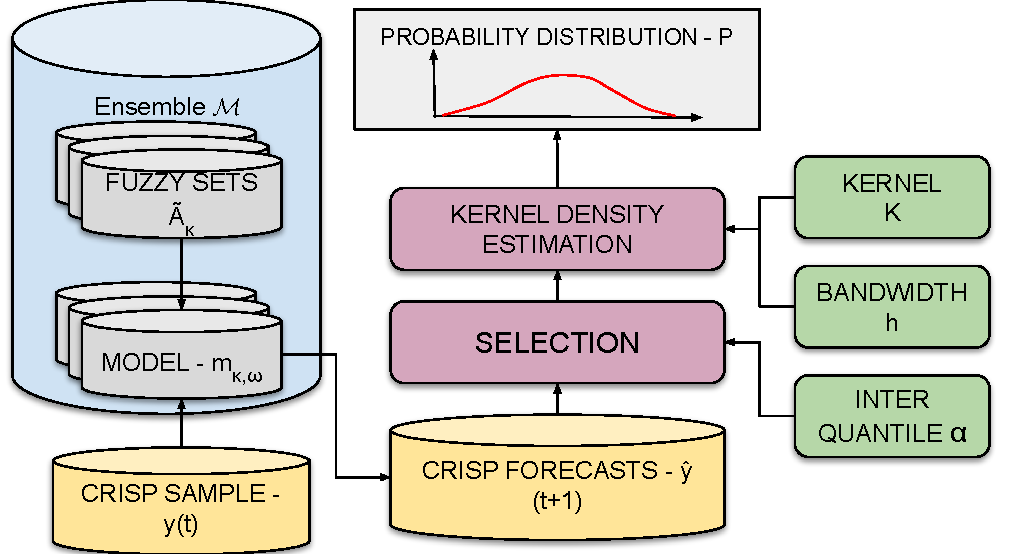
\includegraphics[width=\textwidth]{figures/ensemblefts_forecasting.pdf}
\caption{Ensemble FTS forecasting procedure}
\label{fig:ensemblefts_forecasting}
\end{figure}

%%%%%%%%%%%%%%%%%%%%%%%%%%%%%%%%%%%%%%%%%%%%%%%
\begin{enumerate}

\item[Step 1] \textit{Individual forecasts}: The input sample $y \in Y$ is presented to each internal model $m_j \in \model$, which in turn will produce an individual forecast $\hat{y}_j(t+1)$. The set of crisp forecasts is hereafter called $\hat{y}(t+1)$.

%%%%%%%%%%%%%%%%%%%%%%%%%%%%%%%%%%%%%%%%%%%%%%%
\item[Step 2] \textit{Forecast selection}: In order to control the total forecast variance and eliminate the effect of possible outliers the forecasted output is limited by an inter quantile interval $(\alpha, 1-\alpha)$ where $\alpha \in (0,1)$ is the confidence level. By varying $\alpha$ parameter it is possible to fine tune the final distribution accuracy by eliminating forecasts that are too distant from the mean.

%%%%%%%%%%%%%%%%%%%%%%%%%%%%%%%%%%%%%%%%%%%%%%%
\item[Step 3] \textit{Kernel density estimation}: The set of crisp forecasts $\hat{y}(t+1)$ is used with a kernel density estimator $K$ to estimate the probability distribution $P_{t+1}: U \rightarrow [0,1]$. Two parameters are necessary on this step: the type of kernel and the bandwidth $h$. Both parameters are domain specific and need to be empirically evaluated for each application.
\index{Kernel Density Estimation}\index{KDE}

\index{Many steps ahead forecast}
\item[Step 4] \textit{Many steps ahead forecast}:If the forecasting horizon is $H > 1$, define $P_H = \{P_{t+1}\}$ as the set of intervals and repeat the steps below for each $h=2..H$, otherwise return  $P_{t+1}$.
\begin{enumerate}
    \item[a)]  Find the quantiles $Q = \{.1, .2, .3., .4, .5, .6, .7, .8, .9\}$ of the last $\max(\Omega)$ forecasted sets $\hat{y}(t-\omega)$, $\forall \omega \in \Omega$, such that $\hat{y}_Q(t-\omega) = \{ Q_\tau(\hat{y}(t-\omega) | \tau \in Q)$ where $Q$ is the Quantile Function;
    \item[b)] Apply a Cartesian Product between the quantiles of the last $\max(\Omega)$ forecasted sets, such that $\hat{Y} = \prod_{\omega \in \Omega} \hat{y}_Q(t-\omega)$; 
    \item[c)] Use each sample $\hat{y}(t) \in \hat{Y}$ as input to Step 1 and 2 and aggregate all the results on the set $\hat{y}(t+1)$
    \item[d)] Use $\hat{y}(t+1)$ with Step 3 to produce $P_{t+h}$ and include it on $P_H$. If $h=H$ then return $P_H$.
\end{enumerate}

\end{enumerate}

The probabilistic forecast $P(y(t+1)|y(t))$ aims to represent $\estimate \in U$ uncertainties of the model $\model$ in relation to $k$ and $\Omega$. A sample of the EnsembleFTS for one step and many steps ahead forecasts can be seen in Figures \ref{fig:ensemblefts_sample_onestep} and \ref{fig:ensemblefts_sample_manystep}. 

\begin{figure}[htb]
    \centering
    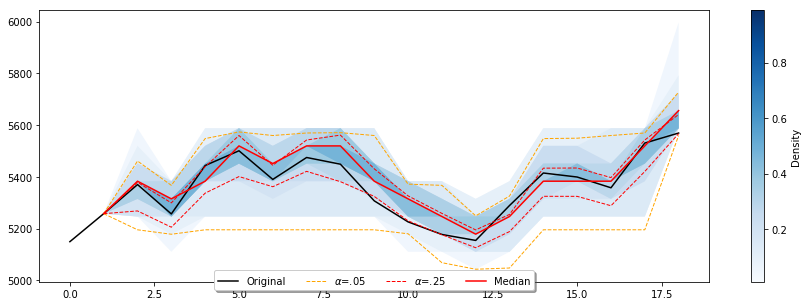
\includegraphics[width=\textwidth]{figures/ensemblefts_sample_onestep.png}
    \caption{Sample of EnsembleFTS performance for one step ahead}
    \label{fig:ensemblefts_sample_onestep}
\end{figure}

\begin{figure}[htb]
    \centering
    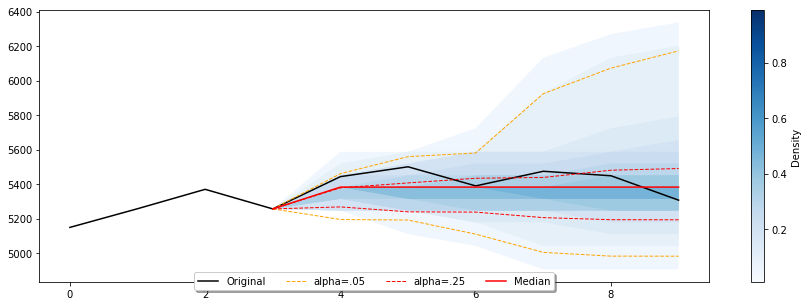
\includegraphics[width=\textwidth]{figures/ensemblefts_sample_manystep.png}
    \caption{Sample of EnsembleFTS performance for many steps ahead}
    \label{fig:ensemblefts_sample_manystep}
\end{figure}

%%%%%%%%%%%%%%%%%%%%%%%%%%%%%%%%%%%%%%%%%%%%%%%%%%%%
%
%%%%%%%%%%%%%%%%%%%%%%%%%%%%%%%%%%%%%%%%%%%%%%%%%%%%
\section{Computational Experiments}\index{Computational Experiments}
\label{sec:prob_experiments}

In this section an empirical study of the performance of the proposed methods is presented using three economic time series. Initially, the datasets, design of experiments and statistical tests employed are discussed. In Section \ref{sec:prob_hyperparameters}, the accuracy sensitivity regarding to the hyperparameters of the proposed methods are analyzed using a grid search. In Section \ref{sec:prob_experiments_interval} the results of the interval forecasting  experiments are presented and discussed and then, in Section \ref{sec:prob_experiments_probabilistic}, the probabilistic forecasting experiments are analyzed.

To measure the performance of the proposed models, ARIMA, QAR, kNN/KDE and, BSTS were chosen as competitor models due to its possibility to perform interval and probabilistic forecasting for many steps ahead. The hyperparameters of each method were individually investigated and only the best model is considered in the validation of the results.

For these experiments three well known financial time series data (the TAIEX, S\&P 500 and NASDAQ data sets) were selected, each of them with 5000 instances, whose descriptions and properties can be found at Appendix \ref{apd:monovariate_datasets}. A rolling window cross-validation methodology \cite{Tashman2000} was applied, using a working set of 1000 instances, 800 for training (80\%) and 200 for testing (20\%) and a sliding increment of 200 instances, totaling 23 experiments, and all measurements were performed out of sample.
\index{TAIEX}\index{S\&P 500}\index{NASDAQ}

Once the model fine tuning was performed for each method and the experiments were executed for each dataset, statistical tests were employed in order to compare the performance of the models. The hypothesis testing procedures adopted best practices discussed in \cite{Garcia2010,Derrac2011,Trawinski2012}. The Friedman Aligned Ranks test \cite{friedmanalignedrankstest} non parametric procedure was adopted to test the equality of the means, where the null hypothesis $H_0$ stands for the equality of all means and the inability to distinguish between the methods and the alternative hypothesis $H_1$ stands for the difference of the means and the distinguishability among the models. The paired \textit{post hoc} procedure adopted was the Finner test \cite{finnertest}, in a one-versus-all design where the proposed methods are taken as control methods. In Finner test  the null hypothesis $H_0$ stands for the equality between the control and the test methods and the alternative hypothesis $H_1$ stands for the significant difference between the control and test methods. All the tests adopted the significance level $\alpha = .05$ and were performed on STAC framework \cite{stac}, and all FTS methods were tested with the pyFTS library\footnote{\url{https://pyfts.github.io/pyFTS/}. Access in 01/07/2018} \cite{pyFTS}. 

In order to contribute to the replication of all the results in the research, all data and source codes employed in this chapter are available at the URL:
\texttt{\url{http://bit.ly/scalable_probabilistic_fts_chapter3}}
\index{Reproducibility}\index{Source codes}

%%%%%%%%%%%%%%%%%%%%%%%%%%%%%%%%%%%%%%%%%%%%%%%%%%%%
%
%%%%%%%%%%%%%%%%%%%%%%%%%%%%%%%%%%%%%%%%%%%%%%%%%%%%
\subsection{Hyperparameter Grid Search}\index{Hyperparameter Grid Search}\index{Hyperparameter Optimization}\index{Hyperparameter}
\label{sec:prob_hyperparameters}

In order to assess the impact of the $\ifts$ and W$\ifts$ methods hyperparameters on the accuracy, a Search Grid was performed for each benchmark dataset, using the search spaces contained in Table \ref{tab:ifts_gridsearch}. The Winkler Score accuracy metric, where  $\alpha \in \{.05,.25\}$, for each method, order, dataset and partitions can be observed in Figures \ref{fig:ifts_gridsearch} and \ref{fig:wifts_gridsearch}. It is notable that $\ifts$ has more sensitivity to the number of partitions than W$\ifts$. This occurs because the length of the partitions is the mechanism used by $\ifts$ method to adjust the importance of each fuzzy set. Otherwise, W$\ifts$ uses the rule weights to balance the importance of each fuzzy set on deffuzyfication, diminishing the impact of the partition length.   

Given that several numbers of partitions and order values achieved very close accuracy values, the Principle of Parsimony (or Occam's Razor) was adopted to choose the set of hyperparameters that leads to smallest number of rules $|\model|$, keeping the same accuracy. The chosen hyperparameters were $k = 45$ and $\Omega = 1$ and a sample of the best models performance can be seen in Figures \ref{fig:ifts_sample_onestep} and \ref{fig:ifts_sample_manystep}.

\begin{table}[htb]
    \centering
    \begin{tabular}{|c|c|c|c|} \hline
        Hyperparameter & Search space  \\ \hline
        $k$ & $\{10, 15, 20, 25, 30, 35, 40, 45, 50\}$  \\ \hline
        $\Omega$ & $\{1, 2, 3\}$ \\ \hline
    \end{tabular}
    \caption{Hyperparameter search spaces for IFTS and WIFTS grid search}
    \label{tab:ifts_gridsearch}
\end{table}

\begin{figure}[htb]
    \centering
    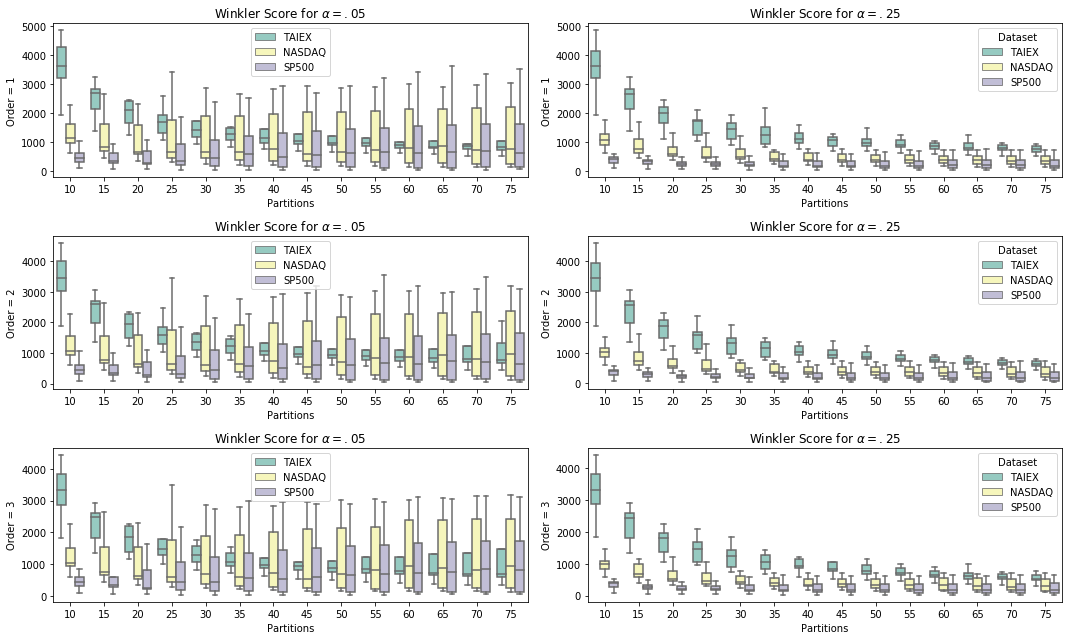
\includegraphics[width=\textwidth,height=15cm]{figures/ifts_gridsearch.png}
    \caption{IFTS Winkler Scores for $\alpha \in \{.05, .25\}$ by dataset, order and partitions}
    \label{fig:ifts_gridsearch}
\end{figure}

\begin{figure}[htb]
    \centering
    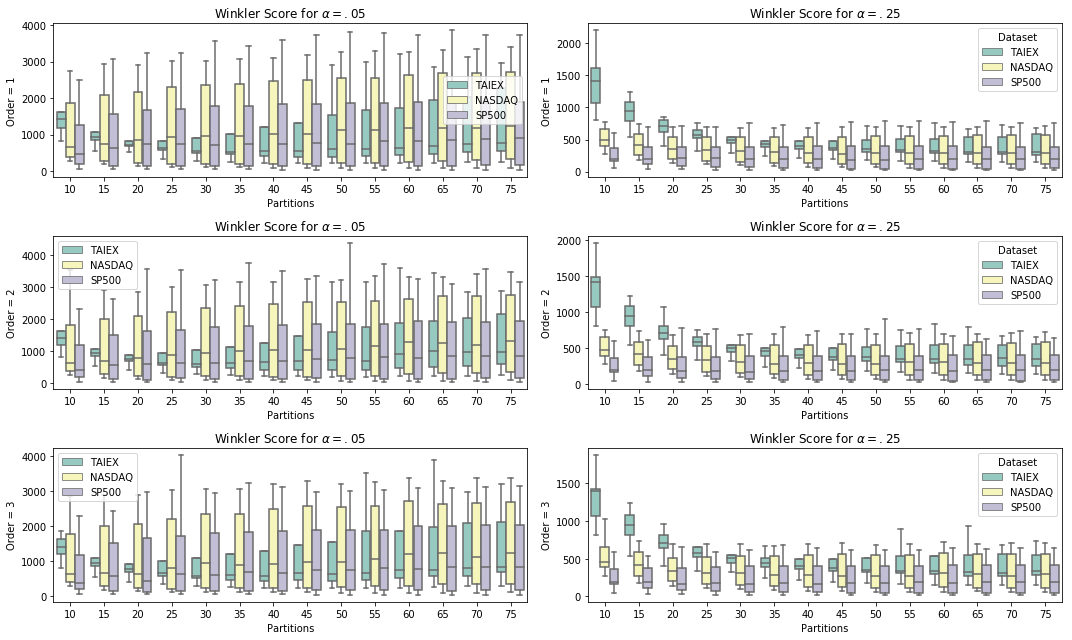
\includegraphics[width=\textwidth,height=15cm]{figures/wifts_gridsearch.png}
    \caption{WIFTS Winkler Scores for $\alpha \in \{.05, .25\}$ by dataset, order and partitions}
    \label{fig:wifts_gridsearch}
\end{figure}

The EnsembleFTS method has a different hyperparameter set than $\ifts$ and W$\ifts$ methods. As a meta-model, an internal FTS model should be chosen, in addition to the $k$ range and the $\Omega$ range. To reduce the complexity of this search space a set of four models were predefined and detailed in Table \ref{tab:ensemblefts_gridsearch}. The accuracy of EnsembleFTS was analyzed using both interval and probabilistic perspectives, the first one using the Winkler Score interval accuracy metric, for  $\alpha \in \{.05, .25\}$, and second one using CRPS probabilistic metric. The Winkler Score for each method and dataset is shown in Figures \ref{fig:ensemblefts_winklerscore}, where can be observed that the Model 4 is the most stable model. The CRPS results are shown in Figure  \ref{fig:ensemblefts_crps}, where it can be observed that Model 4 again is the most stable model. The immediate conclusion is that the higher diversity of models help KDE to build a more precise probability distribution, with improved sharpness and resolution.  A sample of the Model 4 performance can be seen in Figures \ref{fig:ensemblefts_sample_onestep} and \ref{fig:ensemblefts_sample_manystep}, with $\alpha \in \{.05, .25\}$ prediction intervals and probabilistic forecasting for 7 steps ahead.  

\begin{table}[htb]
    \centering
    \begin{tabular}{|c|c|c|c|} \hline
        Name & Internal Model & $k$ range & $\Omega$ range  \\ \hline
        EnsembleFTS Model 1 & HOFTS & $\{10, 20, 30, 40, 50\}$ & $\{1, 2, 3\}$ \\ \hline
        EnsembleFTS Model 2 & HOFTS & $\{10, 15, 20, 25, 30, 35, 40, 45, 50\}$ & $\{1, 2, 3\}$ \\ \hline
        EnsembleFTS Model 3 & WHOFTS & $\{10, 20, 30, 40, 50\}$ & $\{1, 2, 3\}$ \\ \hline
        EnsembleFTS Model 4 & WHOFTS & $\{10, 15, 20, 25, 30, 35, 40, 45, 50\}$ & $\{1, 2, 3\}$ \\ \hline
    \end{tabular}
    \caption{Search spaces for Ensemble FTS grid search}
    \label{tab:ensemblefts_gridsearch}
\end{table}

\begin{figure}[htb]
    \centering
    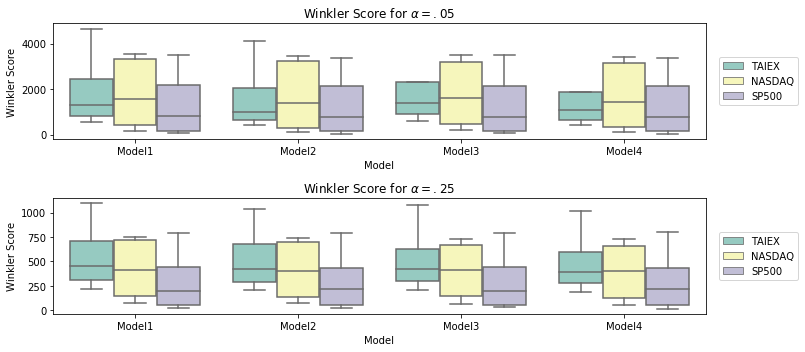
\includegraphics[width=\textwidth]{figures/ensemblefts_winklerscore.png}
    \caption{Sample of IFTS and WIFTS for 7 steps ahead}
    \label{fig:ensemblefts_winklerscore}
\end{figure}

\begin{figure}[htb]
    \centering
    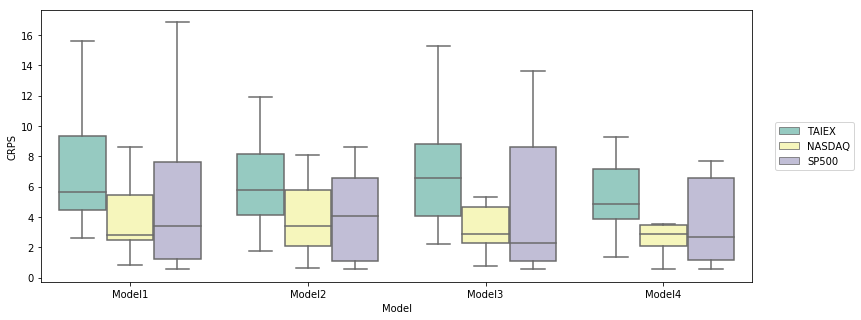
\includegraphics[width=\textwidth]{figures/ensemblefts_crps.png}
    \caption{CRPS response of EnsembleFTS}
    \label{fig:ensemblefts_crps}
\end{figure}

%%%%%%%%%%%%%%%%%%%%%%%%%%%%%%%%%%%%%%%%%%%%%%%%%%%%
%
%%%%%%%%%%%%%%%%%%%%%%%%%%%%%%%%%%%%%%%%%%%%%%%%%%%%
\subsection{Interval Forecasting Benchmarks}\index{Interval Forecasting Benchmarks}
\label{sec:prob_experiments_interval}

The Winkler Score Mean results for each method and dataset are presented in Table \ref{tab:prob_interval_results}. The Friedman Aligned Ranks of the methods are presented in Table \ref{tab:prob_interval_ranks} and the test statistic for these results is $Q = 12.891861761426975$, where the p-Value is $P(\chi^2_{df} < Q) = 0.04478569463323567$, with $df=5$ degrees of freedom. For this statistic the $H_0$ is rejected at the $\alpha=.05$ confidence level, indicating that there is difference between the means of the competitor models.

The \textit{post-hoc} tests were employed using $\ifts$, $W\ifts$ and EnsembleFTS methods as control methods and their results are presented in Tables \ref{tab:prob_interval_posthoc_ifts}, \ref{tab:prob_interval_posthoc_wifts} and \ref{tab:prob_interval_posthoc_ensemblefts}, showing there is no prevalence of the methods except of $W\ifts$ over BSTS. These results showed that $\ifts$, $W\ifts$ and EnsembleFTS interval forecasting methods perform satisfactorily when compared with the standard methods in the literature. 

The statistical tests were employed on the one step ahead forecasts. Figure \ref{fig:interval_many_steps} shows, for each method and dataset, the impact of the forecasting horizon on the Winkler Score accuracy.

\begin{table}[h]
\resizebox{\textwidth}{!}{% <------ Don't forget this %
\centering
    \begin{tabular}{|c|ccccccc|}
\hline
\textbf{Dataset } & \textbf{ ARIMA } & \textbf{ QAR } & \textbf{ WIFTS } & \textbf{ IFTS } & \textbf{ kNN } & \textbf{ EnsembleFTS } & \textbf{ BSTS} \\
\hline
\multirow{2}{*}{S\&P 500} &      72.712 &    121.694 &    111.705 &    113.516 &    131.394 &     268.567 &     292.415 \\
&   $\pm$  135.871 &  $\pm$  319.305 &  $\pm$  156.013 &   $\pm$  91.627 &   $\pm$  166.31 &   $\pm$  318.259 &   $\pm$  384.499 \\ \hline
\multirow{2}{*}{NASDAQ} &     233.261 &    106.416 &     123.35 &    284.692 &    170.709 &     603.881 &     652.036 \\
&   $\pm$  486.735 &   $\pm$  56.248 &  $\pm$  141.251 &   $\pm$  147.24 &  $\pm$  156.097 &   $\pm$  638.297 &   $\pm$  963.624 \\ \hline
\multirow{2}{*}{TAIEX} &     858.124 &        340 &    480.581 &    917.879 &    428.484 &     898.531 &     1280.67 \\
&  $\pm$  1337.139 &   $\pm$  269.34 &  $\pm$  561.826 &  $\pm$  243.737 &  $\pm$  269.459 &  $\pm$  1175.107 &  $\pm$  1472.031 \\ \hline
\end{tabular}
}
    \caption{Average Winkler Score with $\alpha=.05$ for one step ahead interval forecasts}
    \label{tab:prob_interval_results}
\end{table}

\begin{table}[hbt]
    \centering
    \begin{tabular}{|c|c|}
\hline
       \textbf{Rank} &       \textbf{Rank} \\
\hline
          QAR &   5.333333 \\
        WIFTS &   5.666667 \\
          kNN &   6.666667 \\
        ARIMA &  10.000000 \\
         IFTS &  13.666667 \\
  EnsembleFTS &  16.666667 \\
         BSTS &  19.000000 \\
\hline
\end{tabular}
    \caption{Friedman aligned ranks }
    \label{tab:prob_interval_ranks}
\end{table}

\begin{table}[htb]
\resizebox{\textwidth}{!}{% <------ Don't forget this %
    \centering
    \begin{tabular}{|l|c|c|c|c|}
\hline
\textbf{Comparison} &   \textbf{z-Value} &   \textbf{p-Value} &  \textbf{Adjusted p-Value} &       \textbf{Result} \\
\hline
IFTS vs QAR &  1.644879 &  0.099995 &          0.468540 &  H0 Accepted \\
IFTS vs WIFTS &  1.579084 &  0.114317 &          0.468540 &  H0 Accepted \\
IFTS vs kNN &  1.381699 &  0.167064 &          0.468540 &  H0 Accepted \\
IFTS vs BSTS &  1.052723 &  0.292468 &          0.468540 &  H0 Accepted \\
IFTS vs ARIMA &  0.723747 &  0.469221 &          0.532377 &  H0 Accepted \\
IFTS vs EnsembleFTS &  0.592157 &  0.553746 &          0.553746 &  H0 Accepted \\
\hline
\end{tabular}
}
    \caption{Post-hoc tests using IFTS as control method}
    \label{tab:prob_interval_posthoc_ifts}
\end{table}

\begin{table}[htb]
\resizebox{\textwidth}{!}{% <------ Don't forget this %
    \centering
    \begin{tabular}{|l|c|c|c|c|}
\hline
\textbf{Comparison} &   \textbf{z-Value} &   \textbf{p-Value} &  \textbf{Adjusted p-Value} &       \textbf{Result} \\
\hline
WIFTS vs BSTS &  2.631807 &  0.008493 &          0.049889 &  H0 Rejected \\
WIFTS vs EnsembleFTS &  2.171241 &  0.029913 &          0.087081 &  H0 Accepted \\
WIFTS vs IFTS &  1.579084 &  0.114317 &          0.215565 &  H0 Accepted \\
WIFTS vs ARIMA &  0.855337 &  0.392364 &          0.526342 &  H0 Accepted \\
WIFTS vs kNN &  0.197386 &  0.843526 &          0.892023 &  H0 Accepted \\
WIFTS vs QAR &  0.065795 &  0.947541 &          0.947541 &  H0 Accepted \\
\hline
\end{tabular}
}
    \caption{Post-hoc tests using WIFTS as control method}
    \label{tab:prob_interval_posthoc_wifts}
\end{table}

\begin{table}[htb]
\resizebox{\textwidth}{!}{% <------ Don't forget this %
    \centering
    \begin{tabular}{|l|c|c|c|c|}
\hline
\textbf{Comparison} &   \textbf{z-Value} &   \textbf{p-Value} &  \textbf{Adjusted p-Value} &       \textbf{Result} \\
\hline
EnsembleFTS vs QAR &  2.237036 &  0.025284 &          0.142432 &  H0 Accepted \\
EnsembleFTS vs WIFTS &  2.171241 &  0.029913 &          0.142432 &  H0 Accepted \\
EnsembleFTS vs kNN &  1.973855 &  0.048398 &          0.142432 &  H0 Accepted \\
EnsembleFTS vs ARIMA &  1.315903 &  0.188206 &          0.268577 &  H0 Accepted \\
EnsembleFTS vs IFTS &  0.592157 &  0.553746 &          0.620249 &  H0 Accepted \\
EnsembleFTS vs BSTS &  0.460566 &  0.645110 &          0.645110 &  H0 Accepted \\
\hline
\end{tabular}
}
    \caption{Post-hoc tests using Ensemble FTS as control method}
    \label{tab:prob_interval_posthoc_ensemblefts}
\end{table}

\begin{figure}[htb]
    \centering
    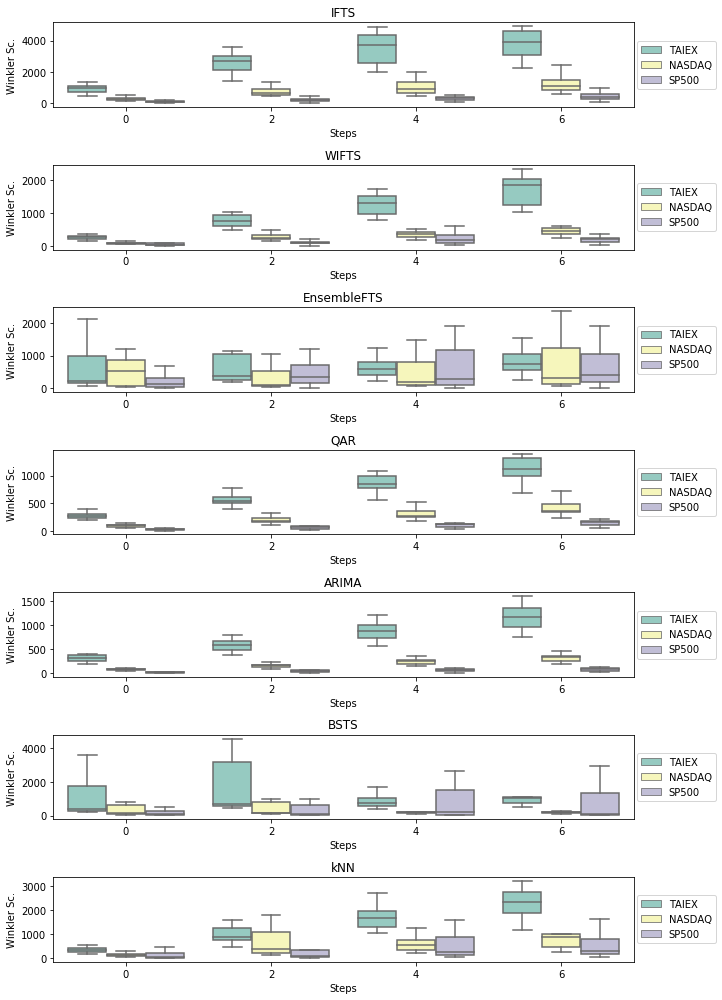
\includegraphics[width=\textwidth]{figures/interval_many_steps.png}
    \caption{Many steps ahead Winkler Score (with $\alpha=.05$) accuracy for each method}
    \label{fig:interval_many_steps}
\end{figure}

%%%%%%%%%%%%%%%%%%%%%%%%%%%%%%%%%%%%%%%%%%%%%%%%%%%%
%
%%%%%%%%%%%%%%%%%%%%%%%%%%%%%%%%%%%%%%%%%%%%%%%%%%%%
\subsection{Probabilistic Forecasting Benchmarks}\index{Probabilistic Forecasting Benchmarks}
\label{sec:prob_experiments_probabilistic}

The CRPS Mean results for each method and dataset are presented in Table \ref{tab:prob_crps_results}. The Friedman Aligned Ranks of the methods are presented in Table \ref{tab:prob_crps_ranks} and the test statistic for these results is $Q = 7.264833574529668$, where the p-Value is $P(\chi ^2_{df} < Q) = 0.12253751253946543$, with $df=4$ degrees of freedom. For this statistic the $H_0$ is accepted at the $\alpha = .05$ confidence level, indicating that there is no difference between the means of the competitor models. This result discards the need to employ \textit{post-hoc} tests and shows that there is no prevalence of one method over others. The EnsembleFTS probabilistic forecasting method performed satisfactorily when compared with the standard methods in the literature. 

The statistical tests were employed on the one step ahead forecasts. Figure \ref{fig:probabilistic_many_steps} shows, for each method and dataset, the impact of the forecasting horizon on the CRPS accuracy.

\begin{table}[htp]
    \centering
    \begin{tabular}{|c|ccccc|}
\hline
\textbf{ Dataset } & \textbf{ QAR } & \textbf{ kNN } & \textbf{ ARIMA } & \textbf{ EnsembleFTS } & \textbf{ BSTS } \\
\hline
\multirow{2}{*}{NASDAQ} &    1.028 &    1.158 &    1.444 &       1.923 &    3.208 \\
&  $\pm$ 0.748 &  $\pm$  0.477 &  $\pm$  1.303 &     $\pm$  1.416 &  $\pm$  3.983 \\ \hline
\multirow{2}{*}{TAIEX} &    1.135 &    1.229 &    1.691 &       1.301 &    4.081 \\
 &  $\pm$  0.613 &  $\pm$  0.693 &  $\pm$  1.239 &     $\pm$  1.118 &  $\pm$  5.306 \\ \hline
\multirow{2}{*}{S\&P 500} &    1.557 &    4.403 &    1.216 &       1.995 &    3.278 \\
&   $\pm$  1.74 &  $\pm$  3.261 &  $\pm$  1.166 &     $\pm$  2.255 &   $\pm$  3.16 \\ \hline
\end{tabular}
    \caption{Average CRPS for one step ahead probabilistic forecasts}
    \label{tab:prob_crps_results}
\end{table}

\begin{table}[htb]
    \centering
    \begin{tabular}{|c|c|}
\hline
\textbf{Method} &  \textbf{Rank} \\
\hline
QAR &   3.000000 \\
ARIMA &   6.666667 \\
kNN &   8.333333 \\
EnsembleFTS &   8.666667 \\
BSTS &  13.333333 \\
\hline
\end{tabular}
    \caption{Friedman Test aligned ranks}
    \label{tab:prob_crps_ranks}
\end{table}

\begin{figure}[htb]
    \centering
    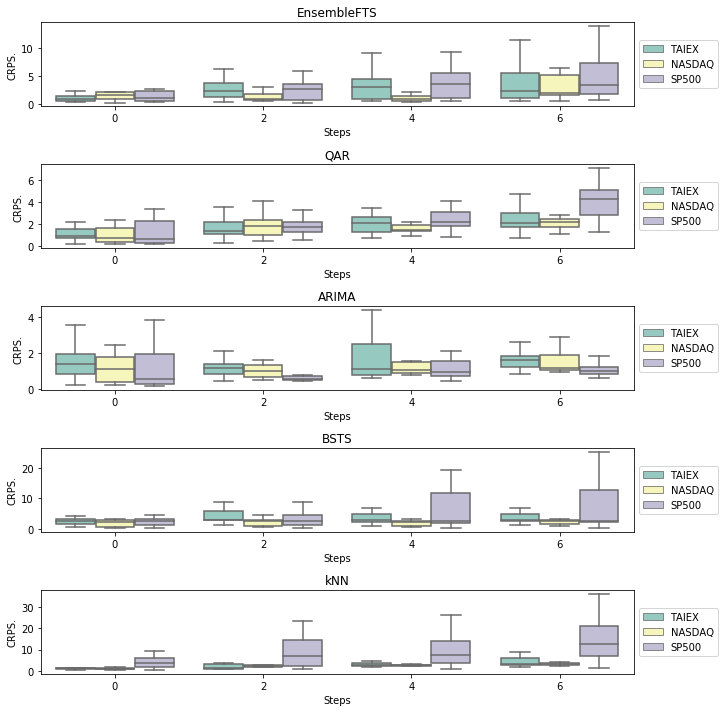
\includegraphics[width=\textwidth]{figures/probabilistic_many_steps.png}
    \caption{Many steps ahead CRPS accuracy for each method}
    \label{fig:probabilistic_many_steps}
\end{figure}


%%%%%%%%%%%%%%%%%%%%%%%%%%%%%%%%%%%%%%%%%%%%%%%%%%%%
%
%%%%%%%%%%%%%%%%%%%%%%%%%%%%%%%%%%%%%%%%%%%%%%%%%%%%
\section{Conclusion}
\label{sec:prob_conclusion}

This chapter provided a brief introduction about point forecasting uncertainties and the main kinds of probabilistic forecasting, reviewing the related literature and proposed new FTS methods for forecasting intervals and probability distributions, which were empirically assessed.

It is remarkable that point forecasts induce to overconfidence and,  without uncertainty measures, point forecasts can be compared to lottery games. It is well known that all forecasting models have an irreducible uncertainty term, besides other not-known or not managed uncertainties, and sometimes this information is critical for decision makers.

The Prediction Interval forecasts allow users to assess the uncertainty, delimiting their expected bounds. Probabilistic forecasting methods assist users to know the uncertainty associated with the entire Universe of Discourse. However, these probabilistic forecasting methods can be computationally expensive and time consuming tasks. Also, the cited models were not adapted to deal with fuzzy numbers as input. The available methods in the FTS literature, at this point, are not capable to forecast prediction intervals or probability distributions.

To exploit this gap it was proposed the Interval FTS - $\ifts$, the Weighted Interval FTS - $W\ifts$, two new FTS approaches to bind the fuzzy uncertainty of the FTS models, and the Ensemble FTS, the first FTS approach capable of to producing probability distributions. In $\ifts$ and $W\ifts$ methods, the prediction interval $\interval$ contains the lower and upper bounds of all fuzzy sets involved on forecasting step, and the length of this interval measures the fuzzy uncertainty.

If $\ifts$ and $W\ifts$ methods deal only with the fuzzy uncertainty, the Ensemble FTS method tries to represent the partitioning and ordering uncertainty to produce probabilistic forecasts. The performed computational experiments showed that the accuracy of the intervals and probability distributions provided by the proposed methods do not differ from the standard methods of the literature, showing its reliability.

\subsection{Methods limitations}\index{Limitations of proposed methods}

The main strength of these methods is their flexibility. These approaches can be used to extend all FTS methods to interval and probabilistic forecasting easily. However, some drawbacks still persist.  $\ifts$ and $W\ifts$ provide intervals, but not probability distributions, and its intervals do not carry a probabilistic uncertainty. Moreover, it is not parsimonious and is computationally expensive when compared to single FTS methods. An integrated method for point, interval and probabilistic forecasting is yet demanded. 

To fix these lacks, in the next chapter a new Fuzzy Time Series method with the ability to  represent epistemic and ontological uncertainty is proposed and its use for point, interval, and probabilistic forecasting is examined.

